\chapter{系统配置:DHCP 和自动配置}
\minitoc
\section{引言}
为了使用TCP/IP协议族,每台主机和路由器需要一定的配置信息。配置信息用于为系
统指定本地名称,以及为接口指定标识符(例如IP 地址)。它还用于提供或使用各种网络服
务,例如域名系统(DNS)和移动IP家乡代理。多年来,已有很多方法可提供和获得这种信
息,但基本上采用3种方法:手工获得信息,通过一个系统获得使用的网络服务,或使用某
种算法自动确定。我们将讨论上述的每种方法,了解它们如何用于 IPv4 和 IPv6。掌握如何
配置系统是很重要的,它是每个系统管理员需要面对的问题,几乎每个终端用户或多或少都
要和它打交道。

我们回忆第2章的内容,TCP/IP 网络中的每个接口都需要一个 IP地址、子网掩码和广
播地址(IPv4)。广播地址通常可通过地址和掩码来确定。系统只要有最基本的信息,就能
与同一子网中的其他系统通信。为了与本地子网之外的系统通信(在第5章中称间接交
付),系统需要一个路由或转发表,以确定到达不同目的地的路由器。为了能够使用某些服
务(例如 Web 和 E-mail),使用DNS(见第11章)将用户可理解的域名映射为低层协议所需
的IP地址。由于 DNS是一个分布式的服务,使用它的任何系统必须知道如何到达至少一台
DNS 服务器。拥有一个IP 地址和子网掩码,以及 DNS服务器和路由器的IP 地址,这是一
个系统能够在 Internet 上运行并提供常用服务(例如 Web 和E-mail)的“基本要素”。为了
使用移动 IP,系统还需要知道如何找到一个家乡代理。

在本章中,我们将主要关注在Internet 客户端主机中用于建立基本要素的协议和程序:
动态主机配置协议(DHCP)以及IPv4 和IPv6 中的无状态地址自动配置。我们还将讨论ISF
如何使用PPP结合以太网来配置客户端系统。服务器和路由器常通过手工配置,通常将相
关配置信息输入一个文件或图形用户界面。这种区别出于以下几个原因。第一,客户端主机
通常比服务器和路由器更容易移动,这意味着应提供灵活的重新分配其配置信息的机制。第
二,服务器主机和路由器都希望“永远可用” 和相对自治。因此,它们的配置信息不依赖于
其他网络服务,能为它们提供更好的可靠性。第三,与服务器或路由器相比,客户机属于某
个组织是更常见的情况,通过一种集中服务来动态分配客户端主机的配置信息,这样将会更
简单也更不容易出错。第四,客户机操作者通常比服务器和路由器管理者拥有更少的系统管
理经验,因此由一个有经验的管理者对多数客户机进行集中管理更不容易出错。

除了上述基本要素之外,主机或路由器的配置信息可能还需要很多其他要素,这取决于
它使用或提供的服务类型。它们可能包括家乡代理、组播路由器、VPN网关和会话发起协议
(SIP)/VOIP 网关的位置。有些服务有标准化的机制和支持协议,以便获得相关的配置信息;
有些服务没有相关的协议,但要求用户输人必要的信息。

\section{动态主机配置协议}
DHCP「RFC21311是一种流行的客户机/ 服务器协议,它用于为主机(有时也为路由器)
指定配置信息。DHCP 在企业和家庭网络中广泛使用,甚至最基础的家庭路由器设备都支持
嵌人式 DHCP 服务器。几乎所有常用的客户端操作系统和大量的嵌入式设备(例如网络打印
机和VoIP电话)都支持DHCP 客户机。这些设备通常使用DHCP 获得IP 地址、子网掩码、
路由器的IP 地址、DNS服务器的IP 地址。其他服务的相关信息(例如使用VOIP 的SIP 服务
器)也可通过DHCP传输。由于 DHCP的最初设想是供IPv4 使用,因此本章中讨论它及其
与IP 的关系时都指的是IPv4版本,除非另外加以说明。IPv6使用的 DHCP 版本是 DHCPV6
\href{https://www.rfc-editor.org/rfc/rfc3315}{\href{https://www.rfc-editor.org/rfc/rfc3315}{[RFC3315]}},我们将在6.2.5节加以讨论,但IPv6 还支持自己的自动程序来确定配置信息。
在一种混合配置模式中,IPv6 自动配置和 DHCPv6可结合使用。

DHCP 的设计基于一种早期协议——称为 Internet 引导程序协议 (BOOTP)\href{https://www.rfc-editor.org/rfc/rfc0951}{\href{https://www.rfc-editor.org/rfc/rfc0951}{[RFC0951]}}
\href{https://www.rfc-editor.org/rfc/rfc1542}{\href{https://www.rfc-editor.org/rfc/rfc1542}{[RFC1542]}},它目前已过时。BOOTP 为客户提供有限的配置信息,并且没有提供一种机制
来支持改变已提供的信息。DHCP 使用租用的概念来扩展BOOTP 模型[GC89],并且可提
供主机操作所需的所有信息。租用允许客户机使用一个商定的时间来配置信息。客户机可向
DHCP服务器请求续订租约,并继续操作。在这个意义上,BOOTP 和DHCP 是向后兼容的,
纯BOOTP 客户端可使用DHCP 服务器,DHCP 客户端也可使用纯BOOTP 服务器。因此,
BOOTP 和 DHCP 同样使用UDP/IP(见第10章)。客户机使用端口 68,服务器使用端口 67。

DHCP 由两个主要部分组成:地址管理和配置数据交付。地址管理用于IP地址的动态分
配,并为客户机提供地址租用。配置数据交付包括 DHCP 协议的消息格式和状态机。DHCP
服务器可配置为提供三种地址分配:自动分配、动态分配和手动分配。三者之间的差异是地
址分配是否基于客户机的身份,以及该地址是否可撤销或变更。最常用方法是动态分配,客
户机从服务器配置的地址池(通常为一个预定义的范围)中获得一个可撤销的IP地址。自动
分配使用的是相同方法,但地址不可撤销。在手动分配中,DHCP 协议用于传输地址,但地址
对于请求的客户机是不变的(即它不是由服务器维护的可分配池的一部分)。在最后一种模式
中,DHCP 的作用如同 BOOTP。我们将专注于动态分配,它是最有趣和最常见的情况。

\subsection{地址池和租用}
在动态分配中,DHCP 客户机请求分配一个IP地址。服务器从可用的地址池中选择一
个地址作为响应。在通常情况下,这个池是专门为 DHCP 用途而分配的一个连续的IP地址
范围。分配给客户机的地址只在一段特定时间内有效,这段时间称为租用期。客户机可使用
这个地址直到租用期到期,尽管它能提出延长租用期的要求。在大多数情况下,客户机可在
希望延长租用期时续订租约。

租用期是 DHCP 服务器的一个重要配置参数。租用期范围可从几分钟到几天或更长时间
(“无限”是可能的,但不推荐这样做,除非是简单的网络)。确定租用期的最佳数值需要对
预期客户数、地址池大小和地址稳定性等因素加以权衡。较长的租用期通常会较快耗尽可用
的地址池,但能提供更稳定的地址和减小网络开销(因续租请求较少)。较短的租用期可
为其他客户提供可用性更高的地址池,随之而来的是稳定性减小和网络流量负荷增大。常见
的默认值包括12~24小时,取决于使用的DHCP 服务器。例如,微软建议较小的网络采用
8天,较大的网络采用16~24天。客户机在租用期过半时开始尝试续订租约。

当发送 DHCP 请求时,客户机需要向服务器提供信息。这些信息可包括客户机名称、请
求的租用期、已使用或最后使用过的地址副本和其他参数。当服务器接收到这个请求时,它
可利用客户机提供的信息(包括MAC地址请求),结合其他从外部获得的信息(例如一天的
时间、接收请求的接口),决定在响应中提供的地址和配置信息。当服务器向客户机提供租
用期时,服务器将租用信息保存在持久性存储器中,通常是非易失性内存或磁盘中。如果
DHCP 服务器重新启动并且运行良好,租约将保持完好。

\subsection{DHCP 和 BOOTP 消息格式}
DHCP 扩展了BOOTP(它是DHCP的前身)。DHCP消息格式的定义采用扩展 BOOTP
的方式,以保持两种协议之间的兼容性,这样即使在没有安装DHCP服务器的网络中,
BOOTP 客户机仍可使用DHCP服务器和BOOTP 中继代理(见6.2.6节)支持DHCP服务。
消息格式包括一个固定长度的初始部分和一个可变长度的尾部(见图6-1)。

图 6-1
BOOTP 消息格式,包括来自\href{https://www.rfc-editor.org/rfc/rfc0951}{\href{https://www.rfc-editor.org/rfc/rfc0951}{[RFC0951]}}、\href{https://www.rfc-editor.org/rfc/rfc1542}{\href{https://www.rfc-editor.org/rfc/rfc1542}{[RFC1542]}}和\href{https://www.rfc-editor.org/rfc/rfc2131}{\href{https://www.rfc-editor.org/rfc/rfc2131}{[RFC2131]}}的字段名。BOOTP 消息格
式采用适当的分配方案保存DHCP 消息。通过这种方式,BOOTP 中继代理可处理DHCP 消息,
BOOTP 客户机可使用 DHCP服务器。如果有必要,服务器名和引导文件名字段可携带 DHCP选项

图6-1所示的消息格式由BOOTP 和DHCP定义在几个 RFC(\href{https://www.rfc-editor.org/rfc/rfc0951}{\href{https://www.rfc-editor.org/rfc/rfc0951}{[RFC0951]}}、\href{https://www.rfc-editor.org/rfc/rfc1542}{\href{https://www.rfc-editor.org/rfc/rfc1542}{[RFC1542]}}和
\href{https://www.rfc-editor.org/rfc/rfc2131}{\href{https://www.rfc-editor.org/rfc/rfc2131}{[RFC2131]}})中。Op(操作)字段标识消息是请求(1)或应答(2)。HW 类型(htype)字段
的分配基于 ARP(见第4章)使用的值,并定义在相应的IANAARP 参数页中[IARP],最常
见的值是1(以太网)。HW 长度(hlen)字段用于存放硬件(MAC)地址,对于类似以太网
的网络,该值通常为6。跳步字段用于保存消息传输过程中的中继次数。消息发送方将该值
设置为0,并在每次中继时递增。事务 ID 是由客户机选择的一个(随机)数,服务器需要将
它复制到响应中。它用于将应答与请求匹配。

秒数(Secs)字段由客户机设置,它是第一次尝试申请或重新申请地址经过的秒数。标
志字段当前只包含一个经过定义的位,称广播标志。客户机可能在请求中设置该位,表示
它们不能或不愿处理单播IP 数据报,但可处理广播数据报(例如,由于它们没有IP地址)。
通过设置该位通知服务器和中继代理,广播地址可用于响应中。

\begin{tcolorbox}
    在 Windows 环境中使用广播标志曾遇到一些困难。Windows XP 和 Windows 7
    的DHCP客户机不能设置该标志,但Windows Vista 的客户机可设置它。在实际使
    用中,有些DHCP服务器不能正确处理该标志,这导致在支持 Vista 客户机时出现
    明显的困难,即使 Vista 实现是 RFC 兼容的。更多信息见[MKB928233]。
\end{tcolorbox}

接下来的四个字段是不同的IP地址。客户机 IP 地址(ciaddr)字段包括请求者的IP地
址(如果已知),否则为0。“你的”IP 地址(yiaddr)字段由服务器填写,以便向请求者提供
服务器地址。下一服务器 IP 地址(siaddr)字段给出下一个服务器的地址,它用于客户机的
引导过程(例如,如果客户机需要下载一个可能需要由 DHCP服务器之外的另一台服务器完
成的操作系统镜像)。网关(中继)IP 地址(giaddr)字段由DHCP或BOOTP 中继器填写,
它们在转发 DHCP(BOOTP)消息时返回自己的地址。客户机硬伴地址(chaddr)字段保存客
户机的唯一标识符,并可由服务器以不同方式来使用,包括当某个客户机每次发送地址请求
时为其分配相同IP地址。这个字段通常保存客户机的MAC地址,它被用作一个标识符。目
前,客户机标识符(6.2.3节和6.2.4节中描述的选项)是它的首选。

其余字段包括服务器名(sname)和引导文件名(file)字段。这些字段并不是每次都需
要填写,它们分别包含64字节或128字节 ASCII 字符,表示服务器名或启动文件路径。这
些字符串以 null 结尾,如同在C编程语言中那样。如果空间紧张(见6.2.3节),它们可用于
保存DHCP选项。最后一个字段最初在BOOTP 中称为供应商扩展字段,其长度固定,现在
称为选项字段,但是长度可变。正如我们将要看到的,选项广泛应用于DHCP 中,以区分
DHCP 消息与传统 BOOTP 消息。

\subsection{DHCP 和 BOOTP选项}
DHCP是对BOOTP的扩展,DHCP 需要的有些字段BOOTP设计之初是不存在的,这
些字段可通过选项来携带。选项采用标准格式,开始以8位标签表示选项类型。对于有些选
项来说,跟在标签后面的固定数量的字节包含选项值。标签构成的所有其他部分之后跟着的
1字节包含选项值长度(不包括标签或长度),紧接着是包含选项值自身的可变数量的字节。

大量选项对于 DHCP 是有效的,其中一些选项也被BOOTP 支持。当前列表由B0OTP/
DHCP参数页[IBDP] 提供。前77个选项包括最常见的选项,它们由\href{https://www.rfc-editor.org/rfc/rfc2132}{\href{https://www.rfc-editor.org/rfc/rfc2132}{[RFC2132]}}定义。常见
选项包括填充(0)、子网掩码(1)、路由器地址(3)、域名服务器(6)、域名(15)、请求
的IP地址(50)、地址租用期(51)、DHCP 消息类型(53)、服务器标识符(54)、参数请求
列表(55)、DHCP 错误消息(56)、租约更新时间(58)、租约重新绑定时间(59)、客户机
标识符(61)、域搜索列表(119)和结束(255)。

DHCP 消息类型选项(53)是1字节长的选项,DHCP 消息一定会使用它,它有以下这些
可能值:DHCPDISCOVER(1)、DHCPOFFER(2)、DHCPREQUEST(3)、DHCPDECLINE(4)、
DHCPACK(5)、DHCPNAK(6)、DHCPRELEASE(7)、DHCPINFORM(8)、DHCPFORCE-
RENEW (9)\href{https://www.rfc-editor.org/rfc/rfc3203}{\href{https://www.rfc-editor.org/rfc/rfc3203}{[RFC3203]}}、DHCPLEASEQUERY(10)、DHCPLEASEUNASSIGNED (11)、
DHCPLEASEUNKNOWN(12)和 DHCPLEASEACTIVE(13)。最后四个值由「RFC43881定义。

选项可由 DHCP 消息中的选项字段携带,也可以由前面提到的服务器名和引导文件名字
段携带。当选项携带在后两个位置时,称为选项超载,将包含一个特殊的超载选项(52)来
表明哪些字段适合携带选项。对于长度超过255字节的选项,\href{https://www.rfc-editor.org/rfc/rfc3396}{\href{https://www.rfc-editor.org/rfc/rfc3396}{[RFC3396]}}定义了一种特殊的
长选项机制。实际上,如果同一选项在同一消息中重复出现多次,它们的内容按出现在消息
中的顺序组合,并将结果作为一个选项来处理。如果一个长选项用于表示选项超载,这时的
处理顺序是从后向前:选项字段、引导文件名字段和服务器名字段。

选项通常提供相对简单的配置信息,或者支持一些其他协商协议。例如,\href{https://www.rfc-editor.org/rfc/rfc2132}{\href{https://www.rfc-editor.org/rfc/rfc2132}{[RFC2132]}}定
义了大多数传统配置信息的选项,传统配置信息指的是 TCP/IP 节点所需的信息(地址信息、
服务器地址、初始TTL 值,以及布尔值指定的配置信息,例如启用IP转发)。下列规范分别
描述了 NetWare 简单配置信息\href{https://www.rfc-editor.org/rfc/rfc2241}{\href{https://www.rfc-editor.org/rfc/rfc2241}{[RFC2241]}}\href{https://www.rfc-editor.org/rfc/rfc2242}{\href{https://www.rfc-editor.org/rfc/rfc2242}{[RFC2242]}}、用户类\href{https://www.rfc-editor.org/rfc/rfc3004}{\href{https://www.rfc-editor.org/rfc/rfc3004}{[RFC3004]}}、FQDN\href{https://www.rfc-editor.org/rfc/rfc4702}{\href{https://www.rfc-editor.org/rfc/rfc4702}{[RFC4702]}}、
Internet 存储名称服务器(iSNS,用于存储网络)\href{https://www.rfc-editor.org/rfc/rfc4174}{\href{https://www.rfc-editor.org/rfc/rfc4174}{[RFC4174]}}、广播和组播服务控制器
(BCMCS,用于3G蜂窝网络)\href{https://www.rfc-editor.org/rfc/rfc4280}{\href{https://www.rfc-editor.org/rfc/rfc4280}{[RFC4280]}}、时区 \href{https://www.rfc-editor.org/rfc/rfc4833}{\href{https://www.rfc-editor.org/rfc/rfc4833}{[RFC4833]}}、自动配置\href{https://www.rfc-editor.org/rfc/rfc2563}{\href{https://www.rfc-editor.org/rfc/rfc2563}{[RFC2563]}}、子网
选择\href{https://www.rfc-editor.org/rfc/rfc3011}{\href{https://www.rfc-editor.org/rfc/rfc3011}{[RFC3011]}}、域名服务选择(见第11章)\href{https://www.rfc-editor.org/rfc/rfc2937}{\href{https://www.rfc-editor.org/rfc/rfc2937}{[RFC2937]}}以及网络接入认证信息承载协议
(PANA)服务器(见第18章)\href{https://www.rfc-editor.org/rfc/rfc5192}{\href{https://www.rfc-editor.org/rfc/rfc5192}{[RFC5192]}}。这些选项用于支持后面(6.2.7节开始介绍)描述
的其他协议和功能。

\subsection{DHCP 协议操作}
DHCP消息是带有一组特殊选项的BOOTP 消息。当一台新的客户机连接到网络时,它
首先发现可用的 DHCP 服务器,以及它们能够提供的地址。然后,它决定使用哪台服务器和
哪个地址,并向提供该地址的服务器发送请求(同时将其选择通知所有服务器)。除非服务
器在此期间已将该地址分配出去,否则它通过确认将地址分配给请求的客户机。图6-2 描述
了典型的客户机和服务器之间事件的时间序列。

一次典型的DHCP 交换。客户机通过广播消息发现一组服务器和可提供的地址,它请求自己想
获得的地址,并接收到选定服务器的确认。交易 ID(xid)用于将请求和响应匹配,服务器1D
(一个选项)指出哪台服务器提供地址,并承诺将它与客户机绑定。如果客户机知道它想获得的
地址,该协议可简化为仅使用 REOUEST 和 ACK 消息

发送请求的客户机将 BOOTP的Op 字段设置 BOOTREQUEST,并将选项字段的前4
字节分别设置为十进制值99、130、83和99(来自\href{https://www.rfc-editor.org/rfc/rfc2132}{\href{https://www.rfc-editor.org/rfc/rfc2132}{[RFC2132]}}的魔术cookie 值)。客户机向
服务器发送消息,使用 UDP/IP数据报,其中包含一个 BOOTP 的 BOOTREQUEST 操作和
相应的DHCP 消息类型(通常 DHCPDISCOVER或 DHCPREQUEST)。这种消息从地址
0.0.0.0(端口 68)发送到受限广播地址 255.255.255.255(端口67)。其他方向(从服务器到
客户机)的消息从服务器IP 地址和端口 67发送到本地IP广播地址和端口68(有关UDP的
详细信息见第10章)。

在一次典型的DHCP 交换中,客户机首先广播一个 DHCPDISCOVER 消息。对于接收
到请求的每台服务器,无论是直接接收还是通过中继代理,它们都会响应一个 DHCPOFFER
消息,并在“你的”IP地址字段中包含提供的IP地址。其他配置选项(例如 DNS服务器的
IP 地址、子网掩码)也经常包括在内。DHCPOFFER 消息中包含租用时间(T),它提供了在
不更新租约的情况下地址可被租用的时间上限。这个消息还包含更新时间(T1),它是客户
机从获得租约到尝试要求服务器更新租约的时间,以及重新绑定时间(T2),它是客户机尝
试要求 DHCP服务器更新其地址的时间。在默认情况下,T1=(T/2),T2=(7T/8)。

当接收到来自一台或多台服务器的DHCPOFFER 消息后,客户机确定自己想接受
哪个 DHCPOFFER,并广播一个包括服务器标识符选项的DHCPREQUEST消息。请求
的IP 地址选项设置为由选中的DHCPOFFER消息提供的地址。多台服务器可能接收到
广播的DHCPREQUEST 消息,但只有 DHCPREQUEST消息中标识的服务器同意将该
地址进行绑定;其他服务器清除与该请求相关的状态。在完成绑定后,选中的服务器响
应一个DHCPACK消息,通知客户机现在可使用该地址。如果服务器无法分配包含在
DHCPREQUEST消息中的地址(例如,已通过其他方式分配或无法使用),该服务器将会响
应一个 DHCPNAK 消息。

当客户机接收 DHCPACK 消息和其他相关的配置信息时,它可探测网络以确保获得的
地址未被使用(例如,向该地址发送一个 ARP 请求以执行 ACD,详见第4章)。如果客户机
确定该地址已被使用,客户机就不使用该地址,并向服务器发送一个 DHCPDECLINE 消息,
通知该地址不能使用。在经过默认的10秒延时后,客户机可重试。如果一台客户机在租约
到期前放弃该地址,它将发送一个 DHCPRELEASE 消息。

在客户机已有一个IP地址并希望仅更新其租约的情况下,它可跳过最初的 DHCPD-
ISCOVER/DHCPOFFER 消息。取而代之的是,客户机通过一个 DHCPREQUEST 消息请求
当前正在使用的地址。此后,协议工作流程如前面所述:服务器可能同意该请求(通过一
个 DHCPACK),也可能拒绝该请求(通过一个 DHCPNAK)。另一种情况,当客户机已有
一个地址时,它不需要更新该地址,但需要其他(非地址的)配置信息。在这种情况下,它
可使用 DHCPINFORM消息来代替DHCPREQUEST 消息,以表明它使用现有地址,但希
望获得额外的信息。这种消息导致服务器返回一个 DHCPACK 消息,其中包括请求的额外
信息。

\subsubsection{例子}
为了观察 DHCP 的行,我们查看一台运行微软 Vista 的笔记本电脑连接到一个无线局
域网时交换的数据包,该网络由一台基于 Linux 的 DHCP 服务器(与Windows 7系统几平相
同)支持。客户机最近使用不同的IP 前缀来访问不同的无线网络,它现在正连接在新的网络
中。由于客户机会记住在之前网络中的地址,它首先尝试通过一个 DHCPREOUEST 消息继
续使用该地址(见图6-3)。

\begin{tcolorbox}
    现在有一个检测网络附件(DNA)的协商过程,分别针对 IPV4\href{https://www.rfc-editor.org/rfc/rfc4436}{\href{https://www.rfc-editor.org/rfc/rfc4436}{[RFC4436]}}和
    IPv6\href{https://www.rfc-editor.org/rfc/rfc6059}{\href{https://www.rfc-editor.org/rfc/rfc6059}{[RFC6059]}}加以规范。这些规范不包含新的协议,而是建议将单播ARP(针对
    IPv4)和单播或多播邻居请求/ 路由器发现消息(针对IPv6,见第8章)相组合,
    它们可在一台主机切换网络链接时减少获取配置信息的延迟。由于这些规范相对较
    新(特别是针对 IPv6),因此并非所有系统都实现了它们。
\end{tcolorbox}


\begin{figure}[H]
    \centering
	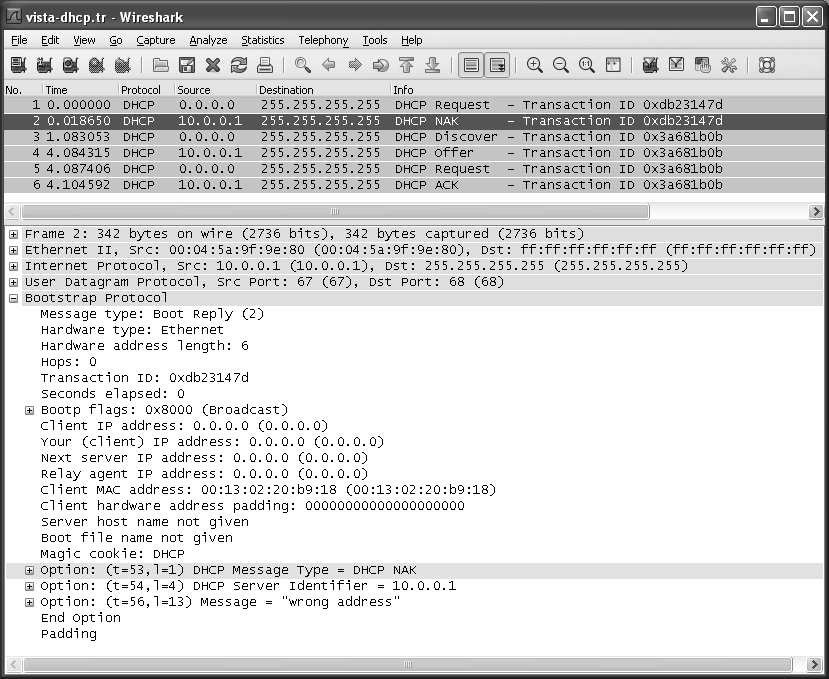
\includegraphics[scale=0.5]{imgs/6/6-4.png}
	\caption{一台客户机已切换网络,但它尝试通过 DHCPREQUEST 消息向新网络中的DHCP 服务器请求自己的旧地址 172.16.1.34}
\end{figure}

在图6-3中,我们可看到用链路层广播帧发送的DHCP 请求(目的地为ff:ff:ff:ff:ff.ff),
它使用未指定的源IP 地址0.0.0.0和受限的广播目的地址 255.255.255.255。由于客户机不知
道请求的地址是否成功分配,也不知道它连接的网络所使用的网络前缀,它将不得不使用这
些地址。这个消息是由 BOOTP 客户机的端口 68(bootpc)向服务器的端口 67(bootps)发送
的UDPAIP数据报。当DHCP作为BOOTP 的一部分时,使用的协议是引导程序协议,消息
类型是 BOOTREQUEST(1),硬件类型设置为1(以太网),地址长度为6字节。事务ID 为
0xdb23147d,它是由客户机选择的一个随机数。这个消息中设置了 BOOTP广播标志,意味
着该消息的响应通过广播地址发送。请求的地址172.16.1.34包含在几个选项之一中。我们
将在 6.2.9节详细介绍 DHCP 消息中出现的选项类型。

附近的DHCP 服务器会接收到客户机的DHCPREOUEST 消息,其中包括请求的IP地
址172.16.1.34。但是,服务器无法分配这个地址,这是由于172.16.1.34不在当前网络中
因此,服务器将会发送一个 DHCPNAK 消息,拒绝客户机的请求(见图 6-4)。

\begin{figure}[H]
    \centering
	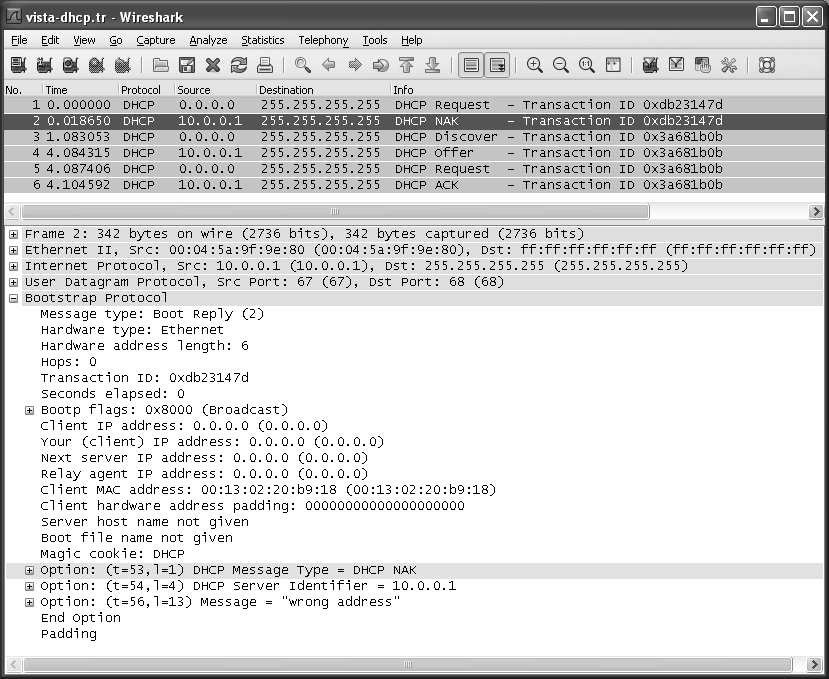
\includegraphics[scale=0.5]{imgs/6/6-4.png}
	\caption{DHCP服务器发送一个 DHCPNAK 消息,表示客户机不应尝试使用 IP 地址 172.16.1.34。事务ID 使客户机知道该消息对应的地址请求}
\end{figure}

图6-4所示的DHCPNAK消息是服务器发送的一个广播BOOTP响应。它包括
DHCPNAK消息类型、与客户机请求匹配的事务ID、包含10.0.0.1 的服务器标识符选
项、客户机标识符(在这种情况下是MAC地址)的副本,以及一个表示错误类型的文
本字符串“wrong address”。此后,客户机不再使用旧地址172.16.1.34,而是通过一个
DHCPDISCOVER 消息(见图6-5)重新寻找它能找到的服务器和地址。

客户机发送的DHCPDISCOVER 消息如图6-5所示,它与DHCPREQUEST 消息相似,
包括之前使用的已请求的IP地址(它没有任何其他要请求的地址),但包含了更丰富的选项
和一个新的事务ID(0x3a681b0b)。除了客户机 MAC地址出现在客户机硬件地址(chaddr)
字段中,大多数主要的 BOOTP 字段保留空并设置0。注意,这个地址如预期那样与以太
网帧的源 MAC地址匹配,这是由于分组并不通过BOOTP 中继代理来转发。DISCOVER 消
息的其他部分包含8个选项,其中大部分在图6-6的屏幕截图中展开了,因此我们可看到多
个选项的子类型。

图6-6给出了BOOTP请求消息中包含的选项。第一个选项表示该消息是一个
DHCPDISCOVER 消息。第二个选项表示客户机是否采用地址自动配置\href{https://www.rfc-editor.org/rfc/rfc2563}{\href{https://www.rfc-editor.org/rfc/rfc2563}{[RFC2563]}}(见 6.3
节)。如果不能通过DHCP 获取地址,则允许它自己决定是否作为 DHCP服务器使用。

\begin{figure}[H]
    \centering
	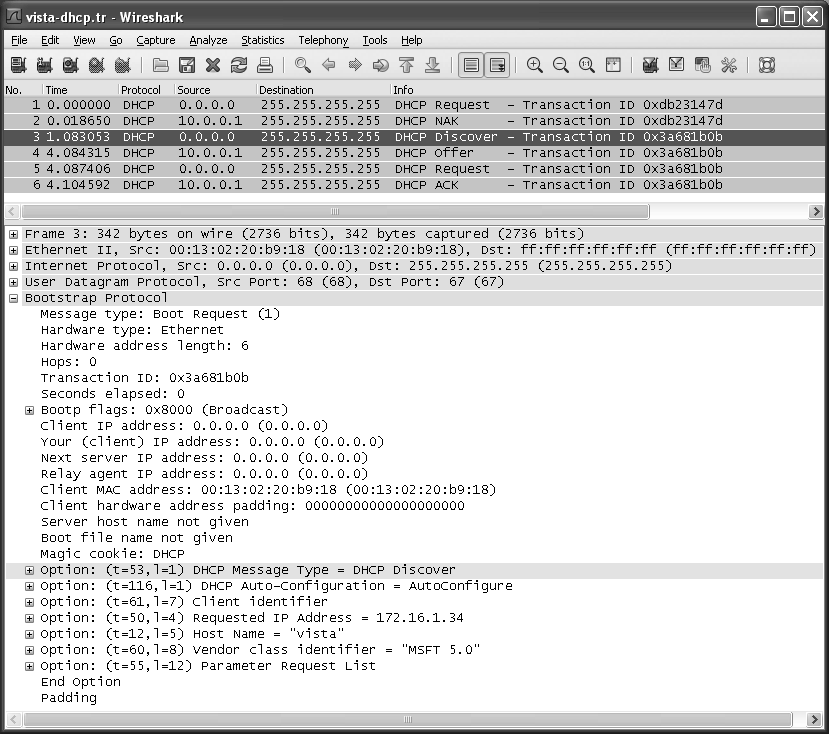
\includegraphics[scale=0.5]{imgs/6/6-5.png}
	\caption{DHCPDISCOVER 消息表明在之前的 DHCPREQUEST 消息失败后,客户机正在重新尝试获得一个地址}
\end{figure}

\begin{figure}[H]
    \centering
	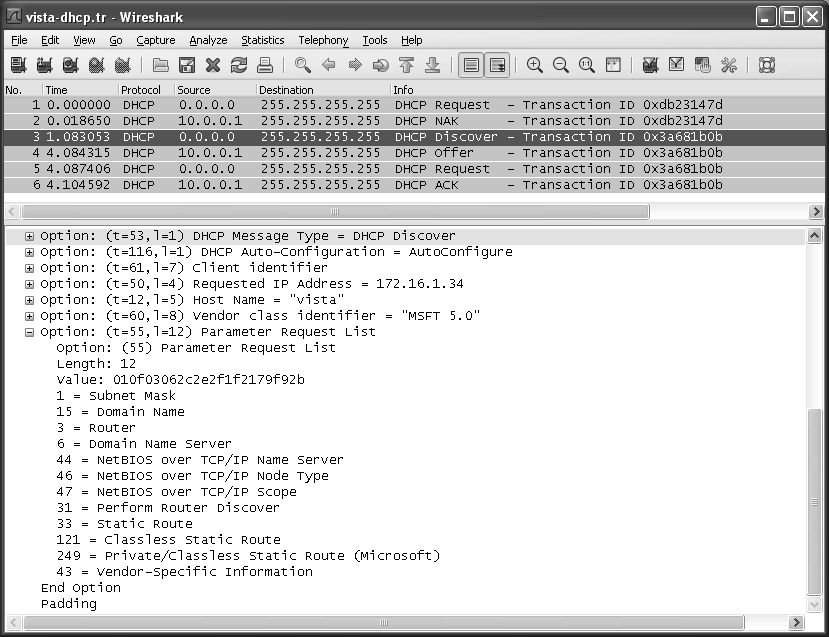
\includegraphics[scale=0.5]{imgs/6/6-6.png}
	\caption{DHCPDISCOVER 消息可能包含丰富的参数请求,说明客户机需要哪些配置信息}
\end{figure}

下一个选项表示客户机标识符(ID)选项设置为0100130220B918(未显示)。DHCP服
务器可使用客户机 ID,以确定是否有特殊配置信息给特定的客户机。目前,大多数操作系
统允许用户在获得一个地址时指定 DHCP 客户机使用的客户机 ID。但是,允许自动选择客
户机 ID 通常更便利,这是由于多个客户机使用相同客户机 ID 会导致DHCP问题。自动选择
的客户机 ID 通常基于客户机MAC地址。在 Windows 中,它是在 MAC地址前面添加一个1
字节的硬件类型标识符(在这种情况下,该字节的值为1,表示以太网)。

\begin{tcolorbox}
    这里出现使用客户机标识符的举动,该标识符并非基于MAC地址。这
    样做的目的是希望一台客户机拥有一个持久的标识符,它使用不变的IPV4或
    IPv6地址,即使系统中的网络接口硬件改变(通常会导致其MAC地址改变)。
    \href{https://www.rfc-editor.org/rfc/rfc4361}{\href{https://www.rfc-editor.org/rfc/rfc4361}{[RFC4361]}}指定了用于IPV4节点的标识符,它使用一种最初为IPV6定义的方
    菜。它涉及使用DHCP 唯一标识(DUID)和身份关联标识符(IAID),它们是为
    DHCPv6\href{https://www.rfc-editor.org/rfc/rfc3315}{\href{https://www.rfc-editor.org/rfc/rfc3315}{[RFC3315]}}(见6.2.5.3节和6.2.5.4节)定义的,但可用于传统 DHCPV4 中。
    它不支持在 DHCP 消息中使用客户机硬件地址(chaddr)字段。但是,这种方案还
    没有被广泛应用。
\end{tcolorbox}

下一个(请求的IP 地址)选项表示客户机请求的IP 地址172.16.1.34。这是它在以前
的无线网络中使用的IP地址。正如前面所述,这个地址在新的网络中无法使用,这是由于
它使用了不同的网络前缀。

其他选项指出了配置主机名“vista”、供应商类别ID“MSFT 5.0”(由 Microsoft
Windows 2000及更高版本系统使用)和一个参数请求列表。参数请求列表选项为DHCP服
务器提供客户机请求的配置信息。它包含一个由多个字节组成的字符串,每个字节表示一个
特定的选项号。我们可以看到,它包含传统 Internet 信息(子网掩码、域名、DNS服务器、
默认的路由器),而且还包含一些其他选项,常见的是针对 Microsoft 系统(即 NetBIOS)的
选项。它还包含一个标识,表明客户机有兴趣知道是否执行 ICMP 路由器发现(见第8章),
以及是否在启动时将静态转发表项添加在客户机的转发表中(见第5章)。

\begin{tcolorbox}
    存在三种静态路由参数是地址发展过程造成的。在全面采用子网掩码和网络
    前缀之前,一个地址的网络部分是需要单独检测的地址(“分类地址”),这是与静
    态路由(33)参数共同使用的路由形式。随着无类路由的使用,DHCP 更新以保持
    掩码可用,这导致了\href{https://www.rfc-editor.org/rfc/rfc3442}{\href{https://www.rfc-editor.org/rfc/rfc3442}{[RFC3442]}}定义的无分类静态路由(CSR)参数(121)的出
    现。微软的改进方案(使用代码249)与之相似。
\end{tcolorbox}

最后一个参数(43)是针对特定供应商的信息。它通常与供应商类别标识符选项(60)
共同使用,以便允许客户机接收非标准的信息。其他方案结合供应商身份与特定供应商信
息\href{https://www.rfc-editor.org/rfc/rfc3925}{\href{https://www.rfc-editor.org/rfc/rfc3925}{[RFC3925]}},提供一种由供应商提供特定信息的方法(即使只有一台客户机)。在采用
Microsoft 系统的情况下,特定供应商信息用于选择使用的 NeBIOS,指出一个 DHCP 租约
是否在关机时释放,以及如何衡量一条默认路由在转发表中的处理。它也可用于 Microsoft
网络访问保护(NAP)系统[MS-DHCPN]。Mac OS 系统使用供应商特定信息支持苹果
NetBoot 服务和引导服务器发现协议(BSDP) [F07]。

在接收一个 DHCPDISCOVER 消息后,DHCP 服务器会响应一个IP 地址、租约和其他
配置信息的确认,它们包含在一个 DHCPOFFER 消息中。在图6-7所示的例子中只有一台
DHCP 服务器(它也是路由器和 DNS服务器)。

\begin{figure}[H]
    \centering
	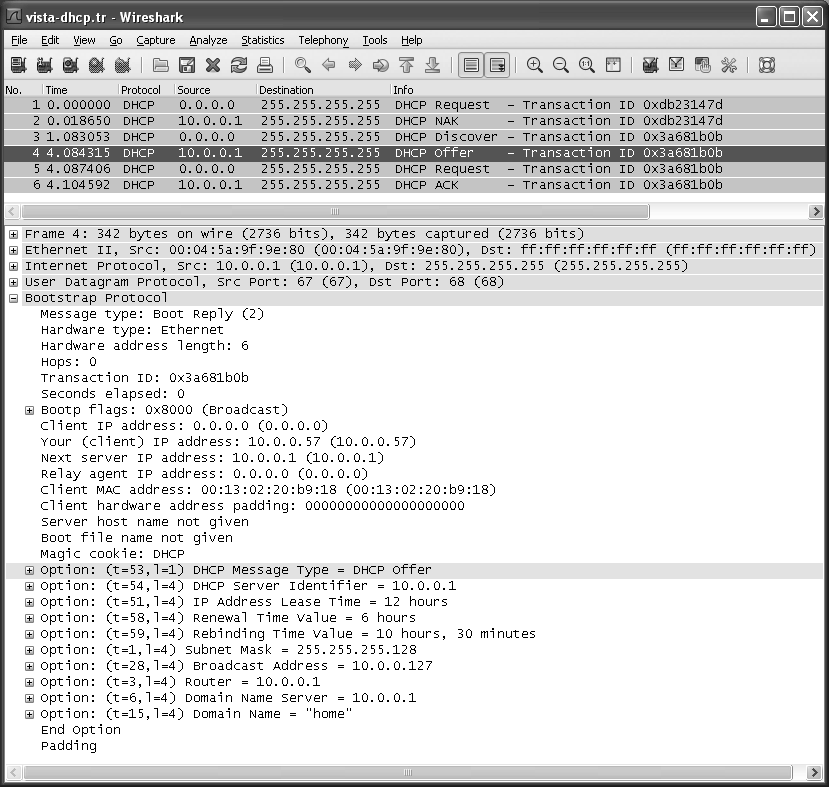
\includegraphics[scale=0.5]{imgs/6/6-7.png}
	\caption{10.0.0.1的DHCP服务器发送的 DHCPOFFER 提供有效期长达12小时的IP 地址10.0.0.57。其
    他信息包括 DNS服务器地址、域名、默认路由器的IP 地址、子网掩码和广播地址。在这个例
    子中,该系统是 IP 地址10.0.0.1 的默认路由器、DHCP 服务器和 DNS服务器}
\end{figure}

在图6-7所示的DHCPOFFER 消息中,我们再次看到消息格式中包含BOOTP 部分,以
及一组涉及DHCP地址处理的选项。BOOTP 消息类型是 BOOTREPLY。由服务器提供的客
户机 IP 地址为10.0.0.57,它位于“你的”[客户机]IP地址字段中。注意,该地址不匹配
DHCPDISCOVER 消息中包含的请求值 172.16.1.34,这是由于 172.16/12 前缀不能用于该本
地网络中。

包含在这组选项中的其他信息包括服务器的IP 地址(10.0.0.1)、提供的IP地址的租用
期(12小时)、T1(更新)和T2(重新绑定)的超时时间(分别为6h和10.5h)。另外,服务
器向客户机提供了子网掩码(255.255.255.128)、正确的广播地址(10.0.0.127)、默认路由
器和 DNS 服务器(均为10.0.0.1,与DHCP服务器一样)和默认域名“home”。该域名在格
式上不是标准的,并且不能用于专用网络之外。这个例子是一个家庭网络,采用作者常用的
<name>.home 格式的机器名。当客户机接收到一个 DHCPOFFER 消息,并决定租用服务岩
提供的 IP 地址10.0.0.57,它会发送第二个 DHCPREOUEST 消息(见图6-8)。

图 6-8
第二个 DHCPREQUEST 表示客户机希望使用IP 地址10.0.0.57。该消息通过广播地址来发送,
并在服务器标识符选项中包含地址10.0.0.1。这样任何其他服务器都可以接收广播,并且知道
客户机选择的 DHCP 服务器和地址

图6-8所示的第二个 DHCPREQUEST 消息与 DHCPDISCOVER消息类似,除了请求的
IP 地址现在设置为10.0.0.57,DHCP 消息类型设置为 DHCPREQUEST,DHCP 自动配置选项
不存在,服务器标识符选项现在已填充了服务器地址(10.0.0.1)。注意,与 DHCPDISCOVER
消息相似,这个消息采用广播方式发送,因此本地网络中的任何服务器或客户机都能接收
它。服务器标识符选项字段用于避免未选中的服务器提交地址绑定。当选中的服务器接收到
DHCPREQUEST 并同意绑定,它通常使用一个 DHCPACK 消息来响应,如图6-9所示。

图6-9所示的DHCPACK消息与前面的DHCPOFFER 消息非常相似。但是,客户机的
FQDN选项现在包括在内。在这种情况下(未显示),它被设置为vista.home。此后,客户机
免费使用地址10.0.0.57,直到 DHCP服务器失效为止。目前,建议使用ACD(在第4章中
描述) 技术,以确保地址不被其他主机使用。

当一个系统启动或连接到一个新的网络时,这个例子中交换的 DHCP 消息是典型的。它
也可能导致一个系统手工释放或获得 DHCP配置消息。例如,在 Windows 中,以下命令将
释放使用 DHCP 获得的数据:

C:\> ipconfig /release

下面的命令将获得数据:

C:> ipconfig /renew

\begin{figure}
    \centering
    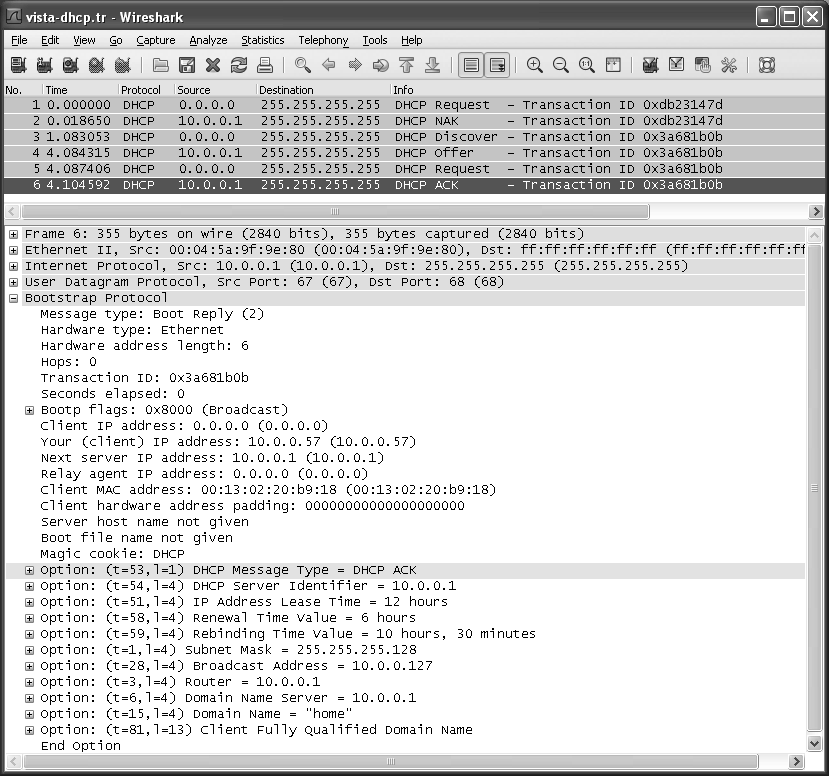
\includegraphics[scale=0.6]{imgs/6/6-9.png}
    \caption{DHCPACK 消息为客户机(和其他服务器)分配地址 10.0.0.57,其有效期长达12小时}
\end{figure}

在Linux 中,以下命令可获得同样结果:

\begin{verbatim}
    
Linux# dhclient -r
\end{verbatim}

释放一个租约,以及
\begin{verbatim}
Linux# dhclient
\end{verbatim}

更新一个租约。

通过DHCP 获得并分配给本地系统的信息类型,可在Windows 中通过一个ipc
选项来查看。下面是来自该命令的一段输出:

\begin{verbatim}
    
C:> ipconfig /a11

Wireless LAN adapter Wireless Network Connection:

Connection-specific DNS Suffix

Description

:home

 :Intel(R)PRO/Wireless 3945ABG

Network Connection

Physical Address... .

:00-13-02-20-B9-18

DHCP Enabled.

Yes

Autoconfiguration Enabled

:Yes

IPV4 Address.....

:10.0.0.57(Preferred)

Subnet Mask



:255.255.255.128

Lease Obtained...





...

:Sunday,December

21,2008

11:31:48 PM

249

250

Lease Expires

:Monday,December 22,2008

11:31:40 AM

Default Gateway

:10.0.0.1

DHCP Server..









:10.0.0.1

DNS Servers..

:10.0.0.1

NetBIOS over Tcpip. 



: Enabled

Connection-specific DNS Suffix Search List :home
\end{verbatim}

这个命令非常有用,可查看通过DHCP 或其他手段为主机分配的配置信息。

\subsection{DHCP状态机}

DHCP 协议在客户机和服务器中运行一个状态机。状态用于指出协议下一个处理的消息类
型。图6-10描述了客户机的状态机。状态之间的转换(箭头)源于消息的接收和发送或超时。

图6-10 DHCP 客户机的状态机。粗体的状态和转换通常涉及客户机首次获得租用地址。虚线和 INIT状
态表示协议开始

如图6-10所示,客户机开始于 INIT(初始)状态,这时没有信息,
并广播 DHCPDISCOVER 消息。在选择状态时,它接收 DHCPOFFER
消息,直到决定自己使用哪个地址和服务器。当它做出选择时,通过
一个 DHCPREQUEST 消息来响应,并进入请求状态。这时,它可能接
收来自不需要的地址的ACK。如果它没有发现需要的地址,发送一
个 DHCPDECLINE 消息,并转换到 INIT 状态。但是,更有可能出现的
情况是,它接收到一个自己需要的地址的DHCPACK 消息,接受它,
获得超时值T1 和T2,并进人绑定状态,这时就能使用这个地址直至
到期。当第一个计时器(T1)到期时,客户机进人更新状态并尝试重新
建立租约。如果它接收到一个新的 DHCPACK(客户机进入绑定状态),
这个过程成功。如果不成功,T2最终到期,并导致客户机尝试从任意服务器重新获得一个
地址。如果租用期最终到期,客户机必须放弃所租用的地址,如果没有可选的地址或可用的
网络连接,这时它将断开网络连接。

\subsection{DHCPV6}
虽然IPv4和IPv6的DHCP 协议希望实现类似目标,但它们各自的协议设计和部署选项
不同。DHCPv6\href{https://www.rfc-editor.org/rfc/rfc3315}{\href{https://www.rfc-editor.org/rfc/rfc3315}{[RFC3315]}} 可使用一种“有状态” 模式,其工作原理非常像DHCPV4,它也
可以使用一种“无状态”模式,并结合无状态地址自动配置(见6.3节)。在无状态模式下,
IPv6 客户机认为自己能配置IPv6地址,但需要通过DHCPv6 获得额外信息(例如 DNS服
务器地址)。另一种选择可使用ICMPv6 路由通告消息(见第8章、第11章和「RFC61061)
获得一台 DNS 服务器的位置。

\subsubsection{IPv6地址生命周期}

IPv6 主机的每个接口通常拥有多个地址,并且每个地址都拥有一组计时器,以指出相应
地址可使用多长时间和用于什么目的。在IPv6 中,地址分配包含一个首选生命周期和一个
有效生命周期。这些生命周期用于判断超时,将地址在自己的状态机中从一种状态转换为另
一种状态(见图6-11)。

图 6-11
IPv6地址的生命周期。临时地址仅用于 DAD,直至被验证为唯一。此后,它们成为首选地
址,并可无限制地使用,直至超时将其状态更改为废弃。废弃地址不能用于初始化新连接,
并且可能在有效超时期满后不能使用

图6-11给出了一个 IPv6地址的生命周期。当一个地址处于首选状态时,它可用于一般
用途,并可作为源或目的IPv6地址。当首选状态的超时到达时,相应的首选地址将废弃。当
该地址处于废弃状态时,它仍可用于现有传输(例如 TCP)连接,但不能用于启动新的连接。

当一个地址第一次被选择使用时,它进人一个临时或乐观状态。在处于临时状态时,它
可能仅用于IPv6邻居发现协议(见第8章)。这时,它不可用作任何其他目的的源或目的地
址。同时,该状态的地址要检测重复,看看同一网络中的其他节点是否已使用该地址。这个
过程称为重复地址检测(DAD),我们将在6.3.2.1 节详细介绍。常规 DAD 的替代方案称
乐观 DAD\href{https://www.rfc-editor.org/rfc/rfc4429}{\href{https://www.rfc-editor.org/rfc/rfc4429}{[RFC4429]}},通过它选择的地址可用于一组有限的用途,直至DAD完成。因为一
个乐观状态的地址实际上仅是针对 DAD 的一组特殊规则,它不是一个真正完整的状态。乐
观地址对大多数目的而言是废弃的。特别是,一个地址可能同时是乐观的和废弃的,这取决
于首选和有效生命周期。

\subsubsection{DHCPv6 消息格式}
DHCPv6消息封装为UDP/IPv6数据报,它使用客户机端口546和服务器端口547(见
第10章)。消息发送到中继代理或服务器,它使用一台主机的链路范围的源地址。这里存在
两种消息格式,一种用于客户机与服务器之间,另一种用于中继代理(见图6-12)。

图6-12左侧给出了基本 DHCPv6消息格式,右侧给出了一种扩展版本,其中包括链
路地址和对等方地址字段。右侧的格式用于 DHCPv6 中继代理和 DHCPv6 服务器之间。链
路地址字段给出了全局 IPv6地址,服务器用它标识客户机所处的链路。对等方地址字段包
含中继代理地址或客户机地址(要中继的消息来自该客户机)。注意,中继过程可能是链状
的,某个中继可能转发来自其他中继的消息。6.2.6节中描述了针对DHCPv4 和 DHCPv6 的
中继

图 6-12
基本 DHCPv6 消息格式(左)和中继代理消息格式(右)。
在DHCPv6中,最有意义的信息携带在选项中

左侧的消息格式中的消息类型包括典型的DHCP 消息(REQUEST、REPLY 等),右侧
的消息格式中的消息类型包括 RELAY-FORW 和 RELAY-REPL,分别表示从中继代理转发和
目的地是中继代理的消息。右侧的选项字段包括一个中继消息选项,其中包含中继转发的完
整消息。其他选项也可包含在内。

DHCPv4 和 DHCPv6之间的区别之一是 DHCPv6使用IPv6 组播地址的方式。客户机将请
求发送到所有 DHCP 中继代理和服务器的组播地址(ff02::1:2)。源地址在链路本地范围。在
IPv6 中,没有保留BOOTP 消息格式。但是,这个消息的语义类似。表6-1给出了 DHCPV6
的消息类型、取值和定义它的RFC,以及针对 DHCPv4 的同类消息和定义它的 RFC。

表6-1 DHCPv6消息的类型、值和标准。右侧给出了针对DHCPV4 的同类消息

DHCPV6 消息

DHCPV6值

参考文献

DHCPv4 消息

SOLICIT

ADVERTISE

REQUEST

CONFFIRM

RENEW

REBIND

REPLY

RELEASE

DECLINE

RECONFIGURE

INFORMATION-REQUEST

RELAY-FORW

RELAY-REPL

LEASEQUERY

\href{https://www.rfc-editor.org/rfc/rfc3315}{\href{https://www.rfc-editor.org/rfc/rfc3315}{[RFC3315]}}

DISCOVER

\href{https://www.rfc-editor.org/rfc/rfc3315}{\href{https://www.rfc-editor.org/rfc/rfc3315}{[RFC3315]}}

OFFER

\href{https://www.rfc-editor.org/rfc/rfc3315}{\href{https://www.rfc-editor.org/rfc/rfc3315}{[RFC3315]}}

REQUEST

\href{https://www.rfc-editor.org/rfc/rfc3315}{\href{https://www.rfc-editor.org/rfc/rfc3315}{[RFC3315]}}

REQUEST

\href{https://www.rfc-editor.org/rfc/rfc3315}{\href{https://www.rfc-editor.org/rfc/rfc3315}{[RFC3315]}}

REQUEST

\href{https://www.rfc-editor.org/rfc/rfc3315}{\href{https://www.rfc-editor.org/rfc/rfc3315}{[RFC3315]}}

DISCOVER

\href{https://www.rfc-editor.org/rfc/rfc3315}{\href{https://www.rfc-editor.org/rfc/rfc3315}{[RFC3315]}}

ACK/NAK

\href{https://www.rfc-editor.org/rfc/rfc3315}{\href{https://www.rfc-editor.org/rfc/rfc3315}{[RFC3315]}}

RELEASE

9

10

11

12

13

14

\href{https://www.rfc-editor.org/rfc/rfc3315}{\href{https://www.rfc-editor.org/rfc/rfc3315}{[RFC3315]}}

DECLINE

\href{https://www.rfc-editor.org/rfc/rfc3315}{\href{https://www.rfc-editor.org/rfc/rfc3315}{[RFC3315]}}

FORCERENEW

\href{https://www.rfc-editor.org/rfc/rfc3315}{\href{https://www.rfc-editor.org/rfc/rfc3315}{[RFC3315]}}

INFORM

\href{https://www.rfc-editor.org/rfc/rfc3315}{\href{https://www.rfc-editor.org/rfc/rfc3315}{[RFC3315]}}

N/A

\href{https://www.rfc-editor.org/rfc/rfc3315}{\href{https://www.rfc-editor.org/rfc/rfc3315}{[RFC3315]}}

N/A

\href{https://www.rfc-editor.org/rfc/rfc5007}{\href{https://www.rfc-editor.org/rfc/rfc5007}{[RFC5007]}}

LEASEQUERY

LEASE{UNASSIGNED,

LEASEQUERY-REPLY

15

\href{https://www.rfc-editor.org/rfc/rfc5007}{\href{https://www.rfc-editor.org/rfc/rfc5007}{[RFC5007]}}

UNKNOWN, ACTIVE}

LEASEQUERY-DONE

LEASEQUERY-DATA

N/A

16

17

N/A

\href{https://www.rfc-editor.org/rfc/rfc5460}{\href{https://www.rfc-editor.org/rfc/rfc5460}{[RFC5460]}}

\href{https://www.rfc-editor.org/rfc/rfc5460}{\href{https://www.rfc-editor.org/rfc/rfc5460}{[RFC5460]}}

N/A

LEASEQUERYDONE

N/A

BULKLEASEQUERY

参考文献

\href{https://www.rfc-editor.org/rfc/rfc2132}{\href{https://www.rfc-editor.org/rfc/rfc2132}{[RFC2132]}}

\href{https://www.rfc-editor.org/rfc/rfc2132}{\href{https://www.rfc-editor.org/rfc/rfc2132}{[RFC2132]}}

\href{https://www.rfc-editor.org/rfc/rfc2132}{\href{https://www.rfc-editor.org/rfc/rfc2132}{[RFC2132]}}

\href{https://www.rfc-editor.org/rfc/rfc2132}{\href{https://www.rfc-editor.org/rfc/rfc2132}{[RFC2132]}}

\href{https://www.rfc-editor.org/rfc/rfc2132}{\href{https://www.rfc-editor.org/rfc/rfc2132}{[RFC2132]}}

\href{https://www.rfc-editor.org/rfc/rfc2132}{\href{https://www.rfc-editor.org/rfc/rfc2132}{[RFC2132]}}

\href{https://www.rfc-editor.org/rfc/rfc2132}{\href{https://www.rfc-editor.org/rfc/rfc2132}{[RFC2132]}}

\href{https://www.rfc-editor.org/rfc/rfc2132}{\href{https://www.rfc-editor.org/rfc/rfc2132}{[RFC2132]}}

\href{https://www.rfc-editor.org/rfc/rfc2132}{\href{https://www.rfc-editor.org/rfc/rfc2132}{[RFC2132]}}

\href{https://www.rfc-editor.org/rfc/rfc3203}{\href{https://www.rfc-editor.org/rfc/rfc3203}{[RFC3203]}}

\href{https://www.rfc-editor.org/rfc/rfc2132}{\href{https://www.rfc-editor.org/rfc/rfc2132}{[RFC2132]}}

\href{https://www.rfc-editor.org/rfc/rfc4388}{\href{https://www.rfc-editor.org/rfc/rfc4388}{[RFC4388]}}

\href{https://www.rfc-editor.org/rfc/rfc4388}{\href{https://www.rfc-editor.org/rfc/rfc4388}{[RFC4388]}}

[ID4LQ]

N/A

[ID4LQ]

在 DHCPv6 中,最有意义的信息携带在选项中,包括地址、租用时间、服务位置,以及
客户端标识符和服务器标识符。这些选项使用的两个重要概念是身份关联(IA)和 DHCP唯
一标识符(DUID)。我们将在后面加以讨论。

\subsubsection{身份关联}
身份关联(IA)是用在DHCP 客户机和服务器之间的一个标识符,用于指向一个地址
集。每个IA 包括一个IA 标识符(IAID)和相关配置信息。每个请求 DHCPv6 分配地址的客
户机接口至少需要一个IA。每个IA 可以仅与一个接口相关联。客户机选择的IAID 唯一地
标识每个IA,并将这个值与服务器共享。

IA 相关的配置信息包括一个或多个地址,以及相关的租约信息(T1、T2和总的租用时
间值)。IA的每个地址都有一个首选的和一个有效的生命周期\href{https://www.rfc-editor.org/rfc/rfc4862}{\href{https://www.rfc-editor.org/rfc/rfc4862}{[RFC4862]}},它定义了地址的
整个生命周期。请求的地址类型可以是常规地址或临时地址\href{https://www.rfc-editor.org/rfc/rfc4941}{\href{https://www.rfc-editor.org/rfc/rfc4941}{[RFC4941]}}。临时地址由随机数
的一部分派生而来,用于协助改善IPv6 主机地址跟踪的隐私问题。临时地址通常与非临时
地址同时分配,但需要频繁使用不同的随机数重新生成。

当服务器响应一个请求时,它客户机的IA 分配一个或多个地址,分配时基于服务器
管理员确定的一组地址分配策略。在通常情况下,这些策略依赖于请求所到达的链路、客
户机的标准信息(见6.2.5.4节的DUID),以及DHCP选项中由客户机提供的其他信息。
图6-13给出了非临时地址和临时地址的IA 选项格式。

0

1516

310

1516

31

OPTION\_IA\_NA

选项长度

OPTION\_IA\_TA

选项长度

IAID(4字节)

T1

T2

IA\_NA 选项

(可变)

针对非临时地址选项的IA

IAID(4字节)

IA\_TA 选项

(可变)

针对临时地址选项的IA

图 6-13
非临时地址(左)和临时地址(右)的DHCPv6 IA 格式。每个选项可能包括额外的选项,以
便描述特定 IPv6 地址和相应的租约

如图6-13所示,对于非临时地址和临时地址的IA选项,主要区别是非临时地址包括
T1 和T2值。这些值是已知的,它们也是DHCPv4使用的值。对于临时地址,可能缺少T1
和T2,因为生命周期通常基于分配给非临时地址的T1 和T2值确定,这些值之前是已知的。
\href{https://www.rfc-editor.org/rfc/rfc4941}{\href{https://www.rfc-editor.org/rfc/rfc4941}{[RFC4941]}}给出了临时地址的细节。

\subsection{ DHCP 唯一标识符}

DHCP 唯一标识符(DUID)用于标识一台 DHCPv6 客户机或服务器,并被设计为可持
续一段时间。服务器用它标识所选地址(作为IA 的一部分)对应的客户机和配置信息,客户
机用它标识感兴趣的服务器。DUID 长度是可变的,对于大多数用途来说,客户机和服务器
将它看作一个不透明的值。

DUID 是全球唯一的,但它很容易生成。为了同时满足这些关系,「RFC33151定义了三
种可能的DUID 类型,但也不是只能创建这三种类型。三种 DUID 类型如下:

1)DUID-LLT:基于链路层地址和时间的 DUID。
2) DUID-EN:基于企业编号和供应商分配的 DUID。
3) DUID-LL:仅基于链路层地址的 DUID。

一个标准格式的DUID编码开始于一个2字节的标识符,用于指出是哪种类型的
DUID。当前列表由IANA维护[ID6PARAM]。在 DUID-LLT 和 DUID-LL 中,紧跟着是一个
来自[RFCO826]的16位的硬件类型;在DUID-EN 中,则是一个32位的专用企业编号。

\begin{tcolorbox}
    专用企业编号(PEN)是一个32位的值,它由IANA 分配给一个企业。它通
    常与 SNMP 协议共同用于网络管理目的。到2011年中期,已分配大约38000个编
    号。当前列表可从IANA 获得[IEPARAM]。
\end{tcolorbox}

第一种格式的 DUID(即 DUID-LLT)是推荐的格式。在硬件类型之后,它包括一个32
位的时间戳,其中的秒数开始于2000年1月1日午夜(UTC)(mod 222)。它将在2136年归
零(返回0)。最后部分是一个可变长度的链路层地址。链路层地址可由任何主机接口选择,
并使用相同的 DUID,一旦选定,它可用于与任何接口的通信。这种格式的DUID 是稳定的,
即使网络接口从该 DUID 中移除。因此,它需要主机系统固定存储相关信息。DUID-LL 格式
非常相似,但推荐给缺少固定存储(但有一个固定的链路层地址)的系统。RFC指出 DUID.
LL 不能用于某些客户机或服务器,它们不能确定自己使用的链路层地址是否与一个可删除
的接口有关。

\subsubsection{协议操作}
DHCPv6协议操作与 DHCPv4 的对应部分相似。一台客户机是否启用 DHCP,取决于这
台主机接收的ICMPv6路由器通告消息中的配置选项(见第8章)。路由器通告包括两个重要
的位字段。M位是可管理地址配置标志,表示IPv6地址可使用DHCPv6 获得。0位是其他
配置标志,表示 IPv6地址之外的其他信息可使用DHCPv6 获得。这两个字段和其他字段定
义在\href{https://www.rfc-editor.org/rfc/rfc5175}{\href{https://www.rfc-editor.org/rfc/rfc5175}{[RFC5175]}}中。M 和O位字段可以任意组合,但M启用和O关闭可能是最不实用的组
合。如果两者都关闭,则不使用DHCPv6,并在分配地址时使用无状态地址自动分配(见6.3
节)。M关闭和O启用表示客户机使用无状态 DHCPv6,并使用无状态地址自动配置获得地
址。DHCPv6协议操作使用表6-1定义的消息,如图6-14所示。

在通常情况下,一台客户机首先确定使用的链路本地地址,然后执行ICMPV6 路由
器发现操作(见第8章),以确定所在网络中是否存在一台路由器。路由器通告包括前面
提到的M和O位字段。如果正在使用DHCPv6,则至少设置M位字段,并且由客户机来
组播(见第9章)DHCPSOLICIT消息,以便发现 DHCPv6服务器。如果存在一个或多个
DHCPADVERTISE 响应消息,表示至少存在一台 DHCPv6服务器。这些消息由2次称为四
消息交换的 DHCPv6操作构成。

在已知一台 DHCPv6服务器位置,或不需要分配地址(例如无状态 DHCPv6 或使用快
速确认选项,见6.2.9节)的情况下,“四消息交换”可简化为“两消息交换”,在这种情况
下只使用请求和应答消息。DHCPv6 服务器确认 DUID、IA 类型(临时、非临时或前缀,见
6.2.5.3节)和IAID结合而成的绑定。IAID 是由客户机选择的一个32位数字。每个绑定可
以有一个或多个租约,一个或多个绑定可通过一个 DHCPv6 事务来处理。

图 6-14
DHCPv6的基本操作。客户机通过ICMPv6路由器通告中的信息决定是否使用DHCPV6。如
果使用,DHCPv6 操作与 DHCPv4 相似,但在细节上有显著不同

\subsubsection{扩展的例子}

图6-15给出了一个例子,一台 Windows Vista (Service Pack 1)机器连接到一个无线网
络。它的IPv4 协议栈已被禁用。它首先分配自己的链路本地地址,并检查该地址是否已被
使用。

在图6-15中,我们看到ICMPv6邻居请求(DAD)为客户机分配的乐观地址为
fe80::fd26:de93:5ab7:405a。(我们在6.3.2.1节讨论无状态地址自动配置时,详细描述了
DAD。)分组发送到对应的目的节点地址 ff02::1:ffb7:405a。它乐观地假设该地址没有在链路
上使用,因此它立即发送一个路由器请求(RS)(见图6-16)。

图6-16中所示的RS发送到所有路由器的组播地址 ff02::2。这导致网络中的每台路由器
都响应一个路由器通告(RA),其中携带重要的M位和O位,客户需要通过它们来决定下一
步怎样做。

\begin{tcolorbox}
    这个例子显示了从乐观地址发送的一个路由器请求,其中包括一个源链路层
    地址选项(SLLAO),这违反了\href{https://www.rfc-editor.org/rfc/rfc4429}{\href{https://www.rfc-editor.org/rfc/rfc4429}{[RFC4429]}}中的规定。这里的问题是对任何处于侦
    听状态的IPv6路由器邻居缓存的潜在污染。它们将处理这个选项,并在自己的邻
    居缓存中建立临时地址和链路层地址之间的映射,这可能重复。但是,这种情况通
    常很少发生,并且不怎么被关注。尽管如此,如果待定的“乐观”选项[IDDN]是
    标准的,将允许路田器请求包含一个用于避免此问题的 SLLAO。
\end{tcolorbox}


\begin{figure}[H]
    \centering
	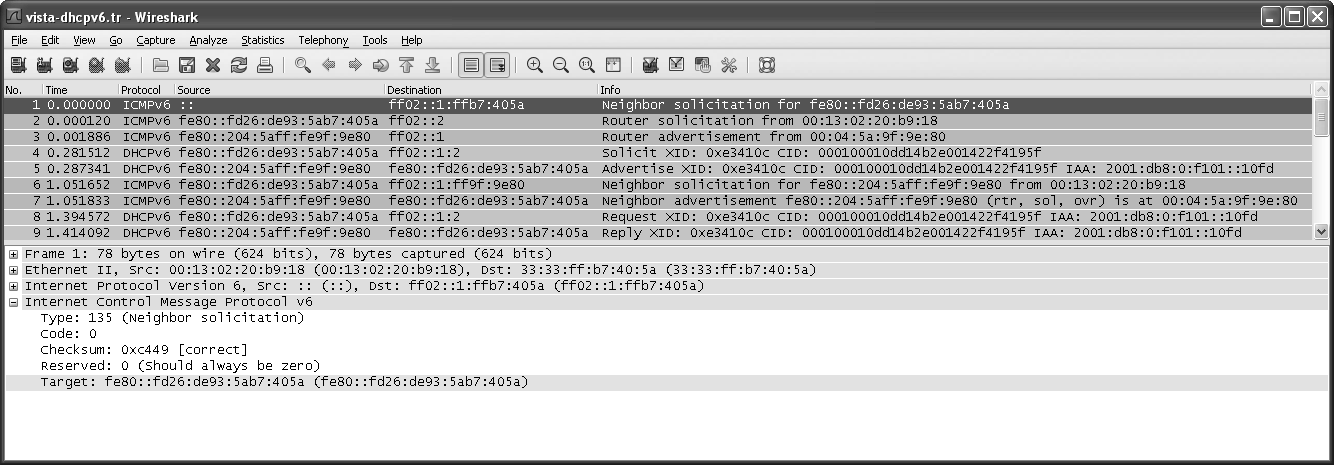
\includegraphics[scale=0.5]{imgs/6/6-15.png}
	\caption{10.0.0.1的DHCP服务器发送的 DHCPOFFER 提供有效期长达12小时的IP 地址10.0.0.57。其
    他信息包括 DNS服务器地址、域名、默认路由器的IP 地址、子网掩码和广播地址。在这个例
    子中,该系统是 IP 地址10.0.0.1 的默认路由器、DHCP 服务器和 DNS服务器}
\end{figure}


\begin{figure}[H]
    \centering
	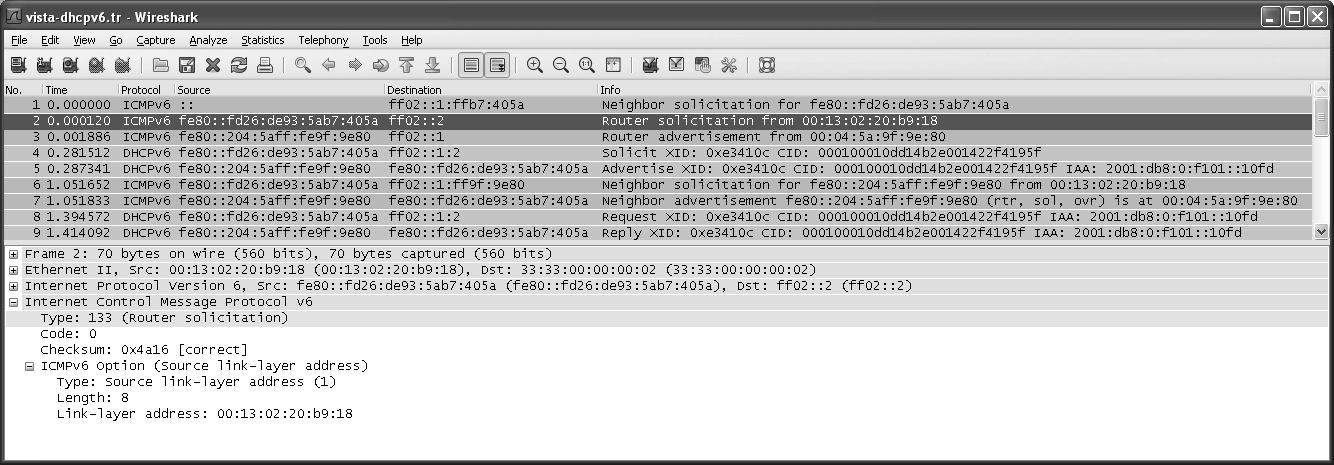
\includegraphics[scale=0.5]{imgs/6/6-16.png}
	\caption{路由器请求导致一台临近的路由器发送了一个路由器通告。请求消息被发送到所有路由器地址(ff02::2)}
\end{figure}

图6-17中的RA表示一台路由器存在,包括00:04:5a:9f:9e:80的 SLLAO,它对客户
机封装目的地为该路由器的后续链路层帧是有用的。标志字段表示M位和O位字段都启用
(设置为1),因此客户机应继续使用DHCPv6,以便获得自己的地址和其他配置信息。这个
过程通过请求一台 DHCPv6服务器来完成(见图6-18)。

\begin{figure}[H]
    \centering
	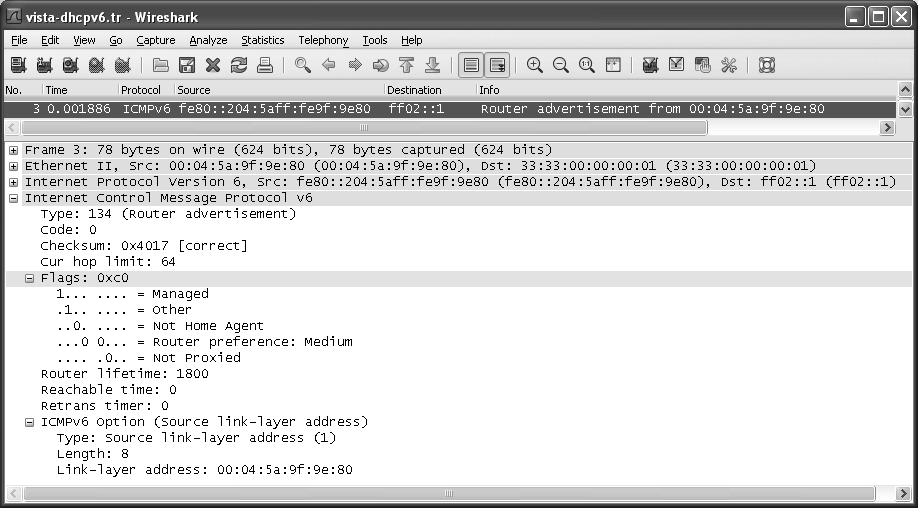
\includegraphics[scale=0.5]{imgs/6/6-17.png}
	\caption{一个路由器通告指出地址可被管理(可使用DHCPv6分配),以及可使用DHCPv6 获得的
    其他信息(例如DNS服务器)。这个网络使用有状态 DHCPv6。IPv6路由器通告消息使用
    ICMPv6(见第8章)}
\end{figure}

图6-18中显示了 DHCPv6 SOLICIT 消息,其中包括事务 ID(与DHCPv4 相似)、经历
的时间(0,图中未显示),以及一个包含时间和6字节MAC地址的DUID。在这个例子中,
MAC地址 00:14:22:f4:19:5f是这台客户机的有线以太网接口MAC地址,它不是用来发送
SOLICIT 消息的接口。回想 DUID-LL 和 DUID-TLL 类型的 DUID,其中的链路层信息对不
同接口应该是一样的。IA是一个非临时的地址,并且客户机已选择IAID 为09001302。这个
请求中的时间值为0,意味着客户机没有特定的期望,它们将由服务器来决定。

下一个选项是\href{https://www.rfc-editor.org/rfc/rfc4704}{\href{https://www.rfc-editor.org/rfc/rfc4704}{[RFC4704]}}规定的FQDN选项。它用于携带客户机的FQDN,但会影响
DHCPv6 和DNS之间的交互(见6.4节中的DHCP 和DNS交互)。这个选项用于启用由客户
机或服务器动态更新的FQDN 到IPv6地址的映射。(反向通常由服务器来处理。)这个选项的
第一部分包含3位:N(服务器不执行更新)、O(服务器忽略客户机请求)和S(服务器执行
更新)。这个选项的第二部分包含一个域名,它可能是完全限定域名,也可能不是。

\begin{tcolorbox}
    Wireshark 工具显示图6-18中记录的FQDN名称异常,并推测该分组可能是
    由一个 MS Vista 客户机生成的。字段异常的原因是这个选项的最初规范允许使用
    ASCII 字符编码的简单域名。这种方法在\href{https://www.rfc-editor.org/rfc/rfc4704}{\href{https://www.rfc-editor.org/rfc/rfc4704}{[RFC4704]}}中已被废弃,并且两种编码不
    直接兼容。微软提供了一个修补程序,为 Vista 系统解决这个问题。微软 Windows
    7系统的行为符合「RFC47041。
\end{tcolorbox}

\begin{figure}[H]
    \centering
	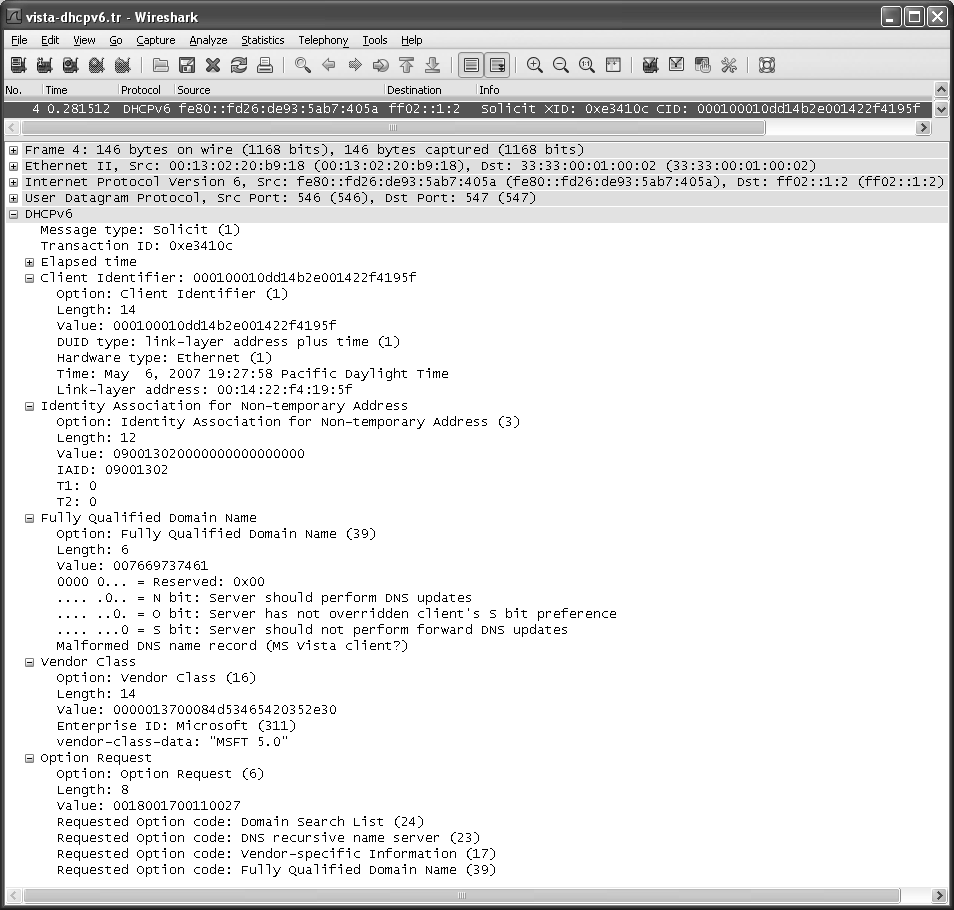
\includegraphics[scale=0.5]{imgs/6/6-18.png}
	\caption{DHCPv6 SOLICIT 消息请求一个或多个 DHCPv6服务器的位置,以及用于识别客户机的信息和它感兴趣的选项}
\end{figure}

请求消息中的其他信息包括供应商类别标识符和请求选项列表。在这种情况下,供应商
类别数据包括字符串“MSFT 5.0”,它可由一台 DHCPv6 服务器使用,以确定客户机能进行
哪些类型的处理。为了响应客户机的请求,服务器响应一个通告消息(见图 6-19)。

图6-19所示的ADVERTISE 消息为客户机提供了更多信息。客户机标识符选项与客户
机配置信息相呼应。服务器标识符选项给出了一个时间和一个链路层地址 10:00:00:00:09:20
来标识服务器。IA拥有一个IAID值09001302(由客户机提供),并包括一个全球地址
2001:db8:0:f101:10fd,其首选生命周期和有效生命周期分别为130s和200s(超时时间相
当短)。状态码为0表示成功。与DHCPv6通告一起提供的还有DNS递归名称服务器选项
\href{https://www.rfc-editor.org/rfc/rfc3646}{\href{https://www.rfc-editor.org/rfc/rfc3646}{[RFC3646]}},它指出一个服务器地址 2001:db8:0:f101::1 和一个包含home 字符串的域名搜索
列表选项。注意,服务器并不包括FQDN 选项,这是由于它不需要执行这个选项。

下面两个分组是常规的邻居请求和邻居通告消息,它们在客户机与路由器之间交
换,我们不会进一步描述它们。这个交换开始于客户机请求确认一个全球非临时地址
2001:db8:0:f101::10fd(见图6-20)。

\begin{figure}[H]
    \centering
	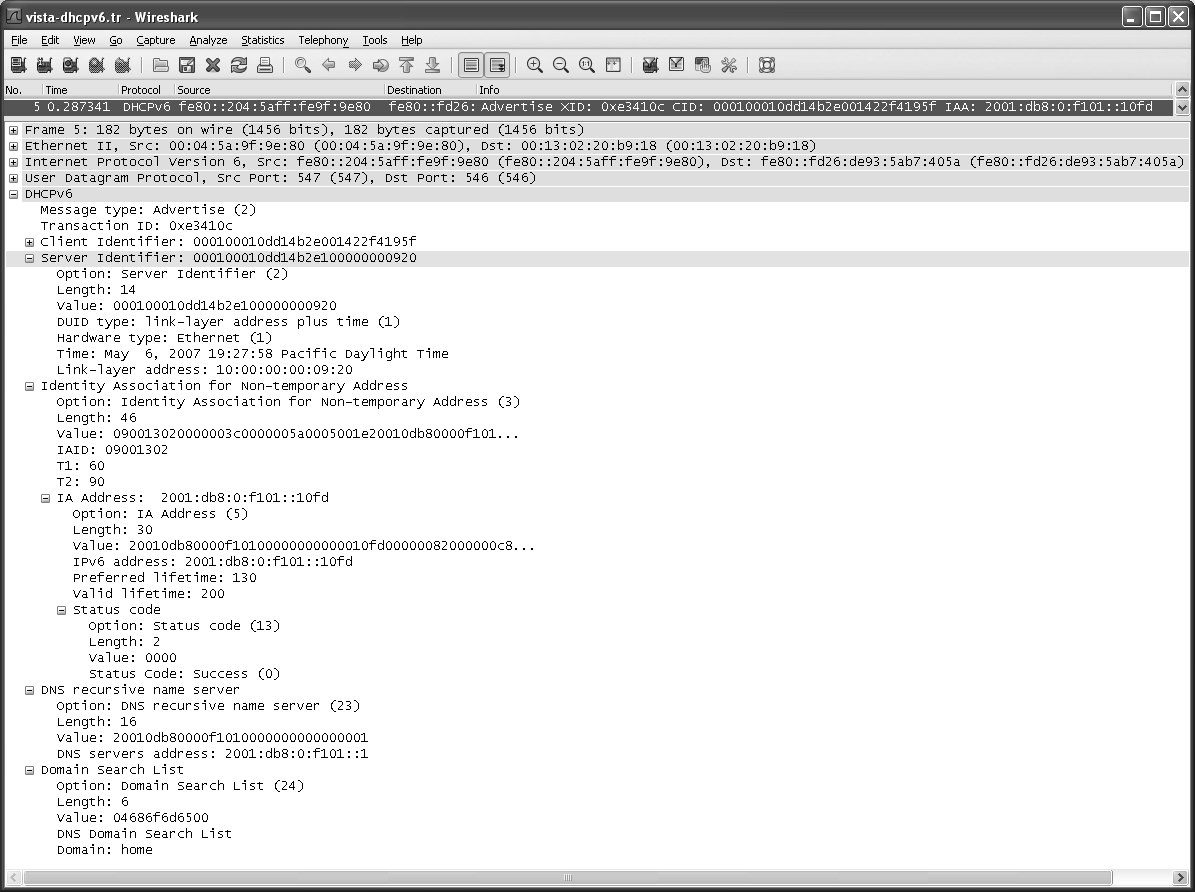
\includegraphics[scale=0.5]{imgs/6/6-19.png}
	\caption{DHCPv6 ADVERTISE 消息包括地址、租约,以及 DNS服务器的IPv6地址和域名搜索列表}
\end{figure}

\begin{figure}[H]
    \centering
	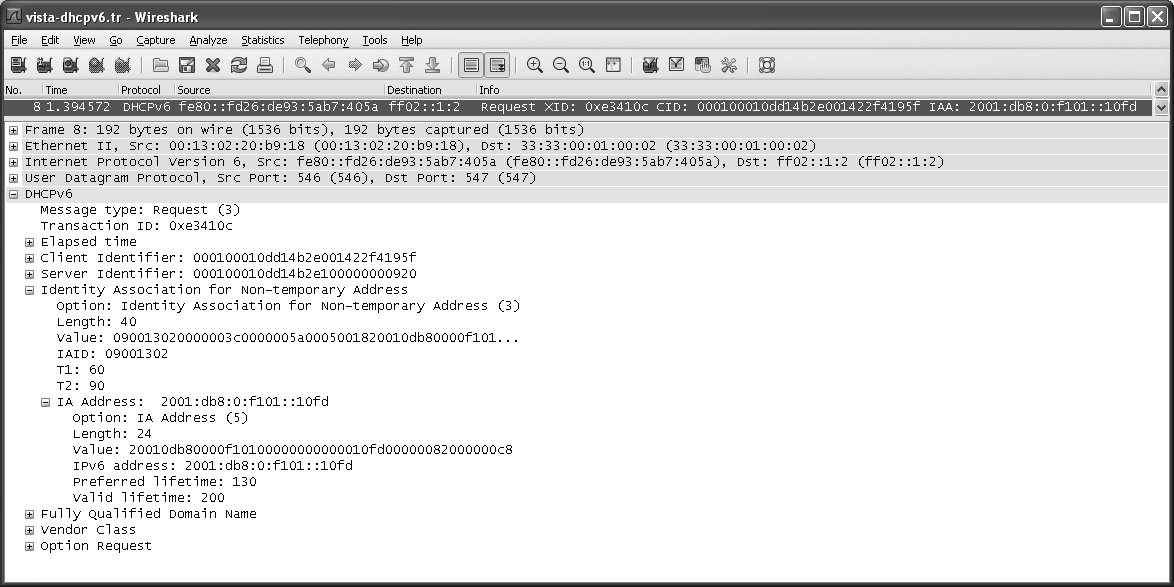
\includegraphics[scale=0.5]{imgs/6/6-20.png}
	\caption{DHCPV6 REQUEST 消息与SOLICIT 消息相似,但它包含从
    服务器 ADVERTISE 消息中学习到的信息}
\end{figure}

图6-20所示的 REQUEST 消息与SOLICIT 消息相似,但它包含来自服务器的 ADVERTISE
消息中携带的信息(地址及T1和T2值)。我们看到的所有 DHCPv6消息中的事务ID 相同。
这个交换通过 REPLY 消息完成,它与ADVERTISE 消息除了消息类型不同之外其余都相同,
因此这里不再详细介绍。

在重启一个系统和连接到一个新的网络时,这个例子中交换的DHCPv6 消息是典型的。
在DHCPv4中,它可能导致一个系统手工释放或获得信息。例如,在 Windows 中,以下命
令使用 DHCPv6 释放获得的数据:

\begin{verbatim}
    C:\> ipconfig /release6
\end{verbatim}

以下命令用于获得它:

\begin{verbatim}
    C:> ipcontig /renew6
\end{verbatim}

通过 DHCP 获得并分配给本地接口的信息类型,可使用之前看过的该命令的另一个选项
来查看。下面是其输出的一部分:
\begin{verbatim}
    C:\> ipconfig /a11

Wireless LAN adapter Wireless Network Connection:

Connection-specific DNS Suffix  :home

Description .

: Intel(R) PRO/Wireless 3945ABG

Network Connection

Physical Address.

DHCP Enabled.

Autoconfiguration Enabled

IPv6 Address.

Lease Obtained.

:00-13-02-20-B9-18

: Yes

:Yes

 : 2001:db8:0:f101::12cd(Preferred)

:Sunday,December 21,2008

11:30:45 PM

Lease Expires

:Sunday,December 21,2008

11:37:04 PM

Link-local IPv6 Address

:

fe80::fd26:de93:5ab7:405a89(Preferred)

Default Gateway .

DHCPv6 IAID



DHCPv6 Client DUID.

: fe80::204:5aff:fe9f:9e8089

:150999810

:

00-01-00-01-0D-D1-4B-2E-00-14-22-F4-19-5F

DNS Servers

:2001:db8:0:f101::1

NetBIOS over Tcpip. .

: Disabled

Connection-specific DNS Suffix Search List :

home

\end{verbatim}
这里,我们可以看到该系统的链路层地址(00:13:02:20:b9:18)。注意,在这个例子中,
该地址从未作形成IPv6 地址的基础而使用。

\subsubsection{DHCPv6 前缀委托(DHCPV6-PD 和ord)}
目前为止的讨论围绕着配置主机,但 DHCPv6也可用于配置路由器。这通过一台路由器
向另一台路由器委托一个地址空间范围来实现。这个地址范围可描述为一个 IPv6地址前缀。
这个前缀在\href{https://www.rfc-editor.org/rfc/rfc3633}{\href{https://www.rfc-editor.org/rfc/rfc3633}{[RFC3633]}}定义的DHCP 前缀选项中。这用于路由器委托的情况,它现在可像一
个 DHCPv6 服务器那样工作,而不需要前缀网络的详细拓扑信息。这种情况可能发生,例如
ISP给出了一个可由潜在客户重新分配的地址范围。在这种情况下,ISP 可能使用 DHCPV6-
PD 向客户设备委托一个前缀。

前缀委托定义了一种新格式的IA,称为IA\_PD。每个IA\_PD 由一个IAID 和相关的配
置信息构成,它在地址上与前面讨论的IA相似。DHCPv6-PD 不只对固定路由器的前缀委托
有用,它也可用于移动路由器(及其连接的子网)[RFC62761。

目前,已创建一种特殊格式的PD(6rd,见\href{https://www.rfc-editor.org/rfc/rfc5569}{\href{https://www.rfc-editor.org/rfc/rfc5569}{[RFC5569]}})以支持服务提供商快速部署
IPv6。在 OPTION\_6RD(212)选项\href{https://www.rfc-editor.org/rfc/rfc5969}{\href{https://www.rfc-editor.org/rfc/rfc5969}{[RFC5969]}}中保存IPv6 6rd前缀,它用于根据客户已分
配的IPv4地址为客户网站分配IPv6地址。IPv6地址是通过算法来分配的,它将服务提供商
提供的6rd前缀作为前n位(推荐n小于32)。客户分配的单播IPv4 地址作为后面的32(或
更少)位,这种IPv6 6rd 委托前缀同样可用DHCPv6-PD 处理,并推荐64位或更短长度用于
自动地址配置(见6.4节)。

OPTION\_6RD 选项长度可变,包括以下几个值:IPv4 掩码长度、6rd前缀长度、6rd 前
缀和6rd 中继地址列表(提供6rd 中继的IPv4地址)。IPv4掩码长度给出了用于分配 IPv6地
址的IPv4 地址位数(从左侧开始计算)。

\subsection{使用 DHCP 中继}
在最简单的网络中,一个 DHCP 服务器可供同一局域网中的客户机使用。但是,在更复
杂的网络中,可通过一个或更多 DHCP 中继代理来中继DHCP 流量,这样做很有必要,而
且可能更方便,如图6-21 所示。

图 6-21
DHCP 中继代理将 DHCP 操作扩展到一个网段之外。中继和 DHCPv4服务器之间的信息可携
带在中继代理信息选项中。DHCPv6 中继以类似的方式工作,但是它拥有一组不同的选项

中继代理用于将 DHCP操作扩展到跨越多个网段。在图6-21 中,网段A和B之间的中
继会转发 DHCP 消息,并通过选项或填充空白字段使用额外信息来标识消息。注意,在一般
情况下,中继不会参与客户机和服务器之间的所有 DHCP 流量交换。相反,它仅中继那些广
播消息(或IPv6 中的组播)。这种消息通常在客户机首次获得自己的地址时交换。当一台客
户机获得一个IP地址,并且服务器的IP 地址使用服务器标识选项时,它可与服务器进行单
播通信而不经过中继。注意,中继代理在传统上是第3层设备,并且通常结合了路由功能。
在讨论第3层中继的基本知识后,我们将简要介绍在第2层的可替代操作。

\subsubsection{中继代理信息选项}
在BOOTP或DHCP 中继的最初概念中\href{https://www.rfc-editor.org/rfc/rfc2131}{\href{https://www.rfc-editor.org/rfc/rfc2131}{[RFC2131]}},中继代理的目的只是将一个消息
从一个子网中继到另一个,而不需要经过一台路由器。这允许系统从一个集中位置不执行
间接传递就获得一个地址。它对于企业基于管理权限进行网络操作是有利的,但在客户采
用DHCP和其他地方(例如 ISP)提供DHCP 基础设施的情况下,这样做有可能需要更多的
信息。这里有很多可能的原因。例如,ISP 可能不完全信任用户,或计费和日志可能与基本
DHCP 协议中没有的其他信息相关。因此,在中继和服务器之间传递的消息中包含额外信息
变得有用。中继代理信息选项(针对 DHCPv4,简称 RAIO)\href{https://www.rfc-editor.org/rfc/rfc3046}{\href{https://www.rfc-editor.org/rfc/rfc3046}{[RFC3046]}}提供了使IPv4 网络
包括这种信息的方法。IPv6 的工作方式不同,我们将在以后章节中介绍。

DHCPv4的RAIO 定义在\href{https://www.rfc-editor.org/rfc/rfc3046}{\href{https://www.rfc-editor.org/rfc/rfc3046}{[RFC3046]}}中,它实际是一个元选项,从某种意义上来说,它
仅定义了一个框架,其中可定义许多子选项。很多这样的子选项已被定义,包括几个被ISP
用于标识一个请求来自哪个用户、链路或网络的选项。在很多情况下,我们看到DHCPv4信
息选项中的每个子选项都有对应的IPv6选项。

由于中继和服务器之间传输的一些信息对安全至关重要,因此在\href{https://www.rfc-editor.org/rfc/rfc4030}{\href{https://www.rfc-editor.org/rfc/rfc4030}{[RFC4030]}}中定义
了RAIO的DHCP认证子选项。它提供了一种确保中继和服务器之间消息交换完整性的方
法。这种方法与 DHCP 延期认证方法非常相似(见6.2.7节),只不过它用SHA-1算法代替了
MDS 算法(见第18章)。

\subsubsection{中继代理远程JD 子选项和IPv6远程ID 选项}
中继的共同需求是通过超出客户机自身提供的信息之外的信息来标识发送 DHCP 请求的
客户机。中继代理信息选项的一个子选项称为远程ID 子选项,它提供了一种标识发送请求
的DHCP 客户机的方法,即采用一系列本地解释的命名方法(例如呼叫方 ID、用户名、调制
解调器ID、一条点到点链路的远程IP 地址)。DHCPv6中继代理远程ID 选项\href{https://www.rfc-editor.org/rfc/rfc4649}{\href{https://www.rfc-editor.org/rfc/rfc4649}{[RFC4649]}}提
供了相同的功能,它还包括一个额外的字段(企业编号),以表明与供应商相关的识别信息。
这种远程ID 信息格式后来以一种基于企业编号的特定供应商方式定义。一种常用的方法是
将 DUID 用于远程ID。

\subsubsection{服务器标识符覆盖}
在某些情况下,中继可能希望干预 DHCP 客户机和服务器之间的操作。这可采用一个
特殊的服务器标识符覆盖子选项来实现\href{https://www.rfc-editor.org/rfc/rfc5107}{\href{https://www.rfc-editor.org/rfc/rfc5107}{[RFC5107]}}。这个子选项是前面提到的 RAIO的一个
选项。

在通常情况下,一个中继会转发SOLICIT消息,并在消息从客户机传递到服务器的过
程中,可能为这些消息附加某些选项。中继在这种情况下是必要的,因为客户机可能还没有
一个可接受的IP 地址,并且仅用广播或组播方式将消息发送到本地子网。当一台客户机接
收并选择自己的地址之后,它可使用服务器标识符选项中携带的服务器标识直接与DHCP服
务器通信。实际上,这将削弱中继在客户机和服务器之间后续事务中的作用。

允许中继为不同类型的消息(例如除了 SOLICT 外的 REQUEST)提供不同选项(例如
RAIO携带一个电路ID),这通常是有用的。这种选项包括一个4字节的值,以指定服务器
生成的 DHCPREPLY 消息中的服务器标识符选项中使用的IPv4地址。服务器标识符覆盖选
项建议与中继代理标志子选项一起使用\href{https://www.rfc-editor.org/rfc/rfc5010}{\href{https://www.rfc-editor.org/rfc/rfc5010}{[RFC5010]}}。这个 RAIO 的子选项是一组标志,它们
可携带从中继到服务器的信息。到目前为止,只有一个关于这种标志的定义:客户机是否使
用广播或单播地址作为初始消息中的目的地址。服务器可能根据这个标志设置做出不同的地
址分配决定。

\subsubsection{租约查询和大批量租约查询}
在某些环境下,允许第三方系统(如中继或接人集中器)学习一个特定DHCP客
户机的地址绑定是有用的。这个功能由DHCP 租约查询(针对 DHCPV4的\href{https://www.rfc-editor.org/rfc/rfc4388}{\href{https://www.rfc-editor.org/rfc/rfc4388}{[RFC4388]}}
\href{https://www.rfc-editor.org/rfc/rfc6148}{\href{https://www.rfc-editor.org/rfc/rfc6148}{[RFC6148]}},或针对DHCPv6的\href{https://www.rfc-editor.org/rfc/rfc5007}{\href{https://www.rfc-editor.org/rfc/rfc5007}{[RFC5007]}})来提供。在DHCPv6中,它也可为委托前缀提
供租约信息。在图6-21中,中继代理可能从经过的DHCP 分组中“搜集”信息,以影响那
些提供给 DHCP服务器的信息。这些信息可能由中继保存,但也可能在中继失败时丢弃。
DHCPLEASEQUERY 消息允许一个代理根据需要重新获得这种信息,它通常发生在一个中
继流量已失去绑定的情况下。对于 DHCPv4,DHCPLEASEQUERY 消息支持4种查询:IPV4
地址、MAC地址、客户机标识符和远程ID。对于 DHCPv6,它支持两种查询:IPv6地址和
客户机标识符(DUID)。

DHCPv4服务器可能用以下几种消息响应租约查询:DHCPLEASEUNASSIGNED、
DHCPLEASEACTIVE或 DHCPLEASEUNKNOWN。第一个消息指出该查询值的响应服务
器是授权的,但目前没有分配相应租约。第二种形式表示一个租约是有效的,并提供了租
约参数(包括T1 和T2)。这里没有对此信息用途的特定建议,无论出于何种目的,都希
望提供给请求者。DHCPv6服务器使用一个 LEASEQUERY-REPLY 消息来响应,其中包含
一个客户机数据选项。这个选项依次包括以下选项:客户机ID、IPv6 地址、IPv6前缀和
客户机的最后事务时间。最后一个值是服务器最后一次询问客户机的时间(以秒为单位)。
LEASEQUERY-REPLY 消息也可包含以下两个选项:中继数据和客户机链路。第一个选项包
括中继最后一次发送的相关查询的数据,第二个选项指出特定客户机拥有一个或多个地址绑
定的链路。再次指出,这个信息可用于请求者希望的任何目的。

租约查询的扩展称为大批量租约查询(BL)\href{https://www.rfc-editor.org/rfc/rfc5460}{\href{https://www.rfc-editor.org/rfc/rfc5460}{[RFC5460]}}[ID4LQ],它可以同时查询多个绑
定关系,使用TCPAIP 而不是UDPAIP,并支持更大范围的查询类型。BL 被设计为一种获得
绑定信息的特定服务,它实际上不是传统 DHCP 的一部分。因此,客户机可能希望不使用
BL 而获得常规配置信息。BL 的一个特用途表现在DHCP 用于前缀委托时。在这种情况下,
最常见的是一台路由器作为一个 DHCP-PD 客户机使用。它获得一个前缀,并从该前缀代表
的一个地址范围中获得一个地址,以分配给传统的DHCP 客户机。但是,如果一台路由器出
现故障或重新启动,它可能会丢失这个前缀信息,并在一段时间内难以恢复,这是因为传统
的租约查询机制需要绑定一个用于查询的标识符。通过扩展一组可能的查询类型,BL 有助
于缓解这种以及其他情况。

BL 提供了对基本租约查询的几个扩展。首先,它使用 TCP/IP(用于 IPv6的端口 547和
用于IPv4的端口67)而不是UDP/IP。这种改变使一次查询可获得大量查询信息,这在检索
大量委托前缀时是必要的。BL也提供了一个中继标识符选项,允许查询者更容易地识别查
询。BL 查询可基于中继标识符、链路地址(网段)或中继ID。

DHCPv6 中继ID选项和DHCPv4 中继ID 子选项[ID4RI]可能包括一个用于标识中继代
理的DUID。中继可在自己转发的消息中插人这个选项,服务器可用它关联自己接收的由特定
中继提供的绑定。BL 支持基于地址和DUID 的查询(定义在\href{https://www.rfc-editor.org/rfc/rfc5007}{\href{https://www.rfc-editor.org/rfc/rfc5007}{[RFC5007]}}和\href{https://www.rfc-editor.org/rfc/rfc4388}{\href{https://www.rfc-editor.org/rfc/rfc4388}{[RFC4388]}}中),也
支持基于中继ID、链路地址和远程ID 的查询。这些新查询只被基于TCP/IP 并支持BL 的服
务器所支持。相反,BL 服务器仅支持 LEASEQUERY 消息,而不是整套的普通 DHCP 消息。

BL 通过 LEASEQUERY-DATA 和 LEASEQUERY-DONE 消息扩展基本的租约查询机制。
当一个查询被成功响应时,一台服务器首先返回一个 LEASEQUERY-REPLY 消息。如果附
加信息是可用的,那么它包括一组 LEASEQUERY-DATA 消息,每个消息对应一个绑定,并
通过一个 LEASEQUBRY-DONE 消息来完成设置。属于相同绑定组的所有消息共享相同的事
务ID,每个相同值由初始的 LEASEQUERY REQUEST 消息提供。

\subsubsection{第2层中继代理}
在一些网络环境中,第2层设备(例如交换机、网桥等)更靠近端系统,它们会中继和
处理 DHCP 请求。这些第2层设备没有完整的TCP/P 协议栈,并且不使用IP进行寻址。因
此,它们不能作为传统的中继代理。为了解决这个问题,[IDL2RA]和\href{https://www.rfc-editor.org/rfc/rfc6221}{\href{https://www.rfc-editor.org/rfc/rfc6221}{[RFC6221]}}分别针对
IPv4 和IPv6规定了第2层“轻量级”DHCP 中继代理(LDRA)如何工作。当针对中继行为
时,接口被标记为面向客户或面向网络,以及可信或不可信。面向网络的接口在拓扑结构上
更接近 DHCP 服务器,可信的接口是那些假设到达的分组不存在欺骗的接口。

IPv4 LDRA的首要问题是如何处理DHCP 的giaddr 字段,以及在LDRA 本身没有IP 层
信息时插人一个 RAIO。[IDL2RA] 推荐的方法是:LDRA 在客户机接收的DHCP 请求中插
入RAIO,但不填写giaddr字段。DHCP 消息以广播方式发送给一个或多个 DHCP 服务器,
以及其他处于接收状态的LDRA。这种消息一直被洪泛(即在所有接口上发送,除了获得该
消息的接口),直到被一个不可信的接口接收。当LDRA接收到一个包含 RAIO 的这种消息,
它不会添加其他的同类选项,但会继续执行洪泛。通过广播发送的响应(例如 DHCPOFFER
消息)可能被LDRA 拦截,这时需要剥离RAIO 并使用其中的信息,以便将响应发送给发出
请求的客户机。很多LDRA 也拦截单播的DHCP 流量。在这些情况下,创建或剥离RAIO
也是必要的。注意,兼容的 DHCP服务器必须支持处理和返回这样的DHCP消息:无论是
用单播发送还是广播发送,其包含的 RAIO 中没有有效的giaddr字段。

IPv6的LDRA 通过创建 RELAY-FORW 和 RELAY-REPL 消息处理DHCPv6流量。面
向客户的接口将会丢弃接收到的 ADVERTISE、REPLY、RECONFIGURE 和 RELAY-REPL
消息。另外,不可信的面向客户的接口也会出于安全原因丢弃接收到的 RELAY-FORW消
息。RELAY-FORW消息包含标识面向客户接口的选项(即链路地址字段、对等方地址字段
和接口ID 选项)。链路地址字段设置为0,对等方地址字段设置为客户机 IP 地址,接口 ID
选项设置为LDRA 中配置的值。当接收到一个链路地址字段为0的 RELAY-REPL 消息时,
LDRA 解封所包含的信息,并将其发送到由接口ID 选项(由服务器提供)指定的客户机接
口。面向客户的接口修改接收的RELAY-FORW 消息的跳步数。面向网络的接口将会丢弃接
收的除 RELAY-REPL 之外的消息。

\subsection{DHCP 认证}
虽然我们通常在每章末尾(正如我们在本章中所做)讨论各种安全漏洞,但在这里提一
下DHCP 的安全问题是值得的。显而易见,如果 DHCP 的顺利运行被干扰,主机很可能配
置为错误的信息,并可能导致严重的服务中断。不幸的是,正如我们已讨论过的那样,DHCP并没有提
供安全保障,因此可能建立一些未授权的DHCP 客户机或服务器,无论是有意的还是无意的,这可能严
重破坏一个网络的其他功能。

DHCP认证选项包括重放检测,可使用不同方法
进行认证。在2001年制定规范时,这个选项没有
像今天这样广泛使用

为了缓解这些问题,\href{https://www.rfc-editor.org/rfc/rfc3118}{\href{https://www.rfc-editor.org/rfc/rfc3118}{[RFC3118]}}规定了一种认证 DHCP 消息的方法。它定义了一个 DHCP选项,即认证
选项,采用如图6-22 所示的格式。

认证选项的目的是确定 DHCP
消息是否来自一个授权的发送方。代码字段设置90,长度字段给出选项中的字节数(不包
括代码或长度字段)。如果协议和算法字段值为0,认证信息字段保存一个简单的共享配置
令牌。只要客户机和服务器的配置令牌匹配,相应的消息可以接收。例如,它可用于保存一
个密码或类似的文本字符串,但这种流量可能被攻击者截获,因此这种方法并不很安全。但
是,它可能有助于抵御偶然的DHCP问题。

一种比较安全的方法称为延期认证,具体看协议和算法字段是否设置为1。在这种情况
下,客户机的DHCPDISCOVER或DHCPINFORM 消息中包含一个认证选项,并且服务器
在 DHCPOFFER 和DHCPACK 消息中包含响应的认证信息。这个认证信息中包括一个消息
认证码(MAC;见第18章),它提供对发送方的认证和消息内容完整性的检验。假设服务器
和客户机有一个共享的密钥,MAC可确保客户机被服务器信任,反之亦然。它也用于确保
客户机和服务器之间交换的 DHCP 消息没有被修改,或是由早期DHCP 消息重放而来。重
放检测方法(RDM)由RDM 字段值来确定。如果 RDM设置为0,重放检测字段包含一个单
向递增的值(例如时间戳)。检测接收的消息以确保该值总是增加。如果这个值没有增加,很
可能是对一个早期DHCP消息的重放(捕获、存储并在此后重新发送)。我们可以想象,在
数据包重新发送的情况下,重放检测字段中的值不会增加。但是,在一个局域网(DHCP 普
遍用于其中)中也可能无法说明问题,这是因为 DHCP 客户机和服务器之间通常只经过一跳
路由。

DHCP 认证没有广泛使用(至少)有两个原因。第一,这种方法需要在 DHCP 服务器和
每个需要认证的客户机之间分发共享密钥。第二,认证选项的定义出现在DHCP 已广泛使用
之后。尽管如此,\href{https://www.rfc-editor.org/rfc/rfc4030}{\href{https://www.rfc-editor.org/rfc/rfc4030}{[RFC4030]}}建立在这个规范之上,以帮助DHCP 消息通过中继代理安全转
发(见6.2.6节)。

\subsection{重新配置扩展}
在普通操作中,DHCP 客户机启动对地址绑定的更新。\href{https://www.rfc-editor.org/rfc/rfc3203}{\href{https://www.rfc-editor.org/rfc/rfc3203}{[RFC3203]}}定义了重新配置扩
展和相关的 DHCPFORCERENEW消息。这个扩展允许服务器引发一个客户机改变更新状
态,并通过别的普通操作(即 DHCPREQUEST)尝试更新租约。一台不希望更新租约的服务
器可能响应一个 DHCPNAK,导致客户机重新启动为 INIT 状态。这台客户机稍后使用一个
DHCPDISCOVER 消息重新开始。

这个扩展的目的是当网络中出现一些明显的状态改变时,使客户端能重新建立一个地址
或丢弃自己的地址。例如,如果网络在管理中关闭或重新编号,这种情况很可能会发生。由
于这种消息经常被 DoS攻击所利用,因此它必须通过DHCP 认证加以验证。由于DHCP 认
证没有得到广泛使用,因此重新配置扩展同样没有流行起来。

\subsection{快速确认}
DHCP 快速确认选项\href{https://www.rfc-editor.org/rfc/rfc4039}{\href{https://www.rfc-editor.org/rfc/rfc4039}{[RFC4039]}}允许一台 DHCP服务器通过一个 DHCPACK 来响应
DHCPDISCOVER 消息,从而有效跳过DHCPREQUEST消息,并最终使用两消息交换
来代替四消息交换。这个选项的设计目的是快速配置可能频繁改变其网络接人点的主机
(例如移动主机)。当仅有一台可用的DHCP服务器并且地址充足时,我们可以不关注这
个选项。

要使用快速确认,客户机可在 DHCPDISCOVER 消息中包含该选项,但在任何其他消
息中不能包含该选项。同样,服务器仅在 DHCPACK 消息中使用该选项。当一台服务器使用
该选项来响应时,接收消息的客户机知道该返回地址可立即使用。如果后来确定该地址已用
于另一个系统(例如通过ARP),客户机发送一个 DHCPDECLINE 消息,并放弃该地址。客
户机也可能通过一个 DHCPRELEASE 消息自愿放弃接收到的地址。

\subsection{位置信息(LCI 和 LoST)}

在某些情况下,将主机配置为知道自己的位置是有用的。这样的信息可编码使用,例如
纬度、经度和海拔高度。IETF 的一个众所周知的成果是 Geoconf(“地理配置”)\href{https://www.rfc-editor.org/rfc/rfc6225}{\href{https://www.rfc-editor.org/rfc/rfc6225}{[RFC6225]}},
\href{https://www.rfc-editor.org/rfc/rfc6225}{\href{https://www.rfc-editor.org/rfc/rfc6225}{[RFC6225]}}规定了如何使用GeoConf(123)和 GeoLoc(144)的DHCP选项,为客户机提供
这种地理空间位置配置信息(LCI)。地理空间LCI 不仅包括纬度、经度和高度坐标,也为每
个信息提供分辦率指标。LCI 可用于一系列目的,包括紧急服务。如果一个呼叫者使用IP 电
话请求紧急援助,LCI 可指示发生紧急情况的位置。

尽管刚提到的物理位置信息对找到特定的个人或系统是有用的,但有时知道一个实体的
市政位置也是重要的。市政位置根据行政地理表示位置,例如国家、城市、区、街道,以及
其他类似的参数。市政位置信息可通过DHCP以物理位置所采用的方式提供,使用的LCI
结构与地理空间LCI 中使用的一样。\href{https://www.rfc-editor.org/rfc/rfc4776}{\href{https://www.rfc-editor.org/rfc/rfc4776}{[RFC4776]}}定义了携带市政位置的GEOCONF\_CIVIC
(99)选项。这种格式的LCI 比地理空间信息更麻烦,这是因为各个国家在行政地理上命名
位置的方法不同。由于这种名称除了需要 DHCP 常用的英语、ASCII语言和字符集外,可能
还需要其他语言和字符集的支持,这会带来额外的复杂性。不仅是 DHCP 方面,这里还存
在位置的隐私问题。IETF 在 Geopriv 框架中讨论了这个问题。例如,参见\href{https://www.rfc-editor.org/rfc/rfc3693}{\href{https://www.rfc-editor.org/rfc/rfc3693}{[RFC3693]}}了解
更多信息。

一个可供选择的高层协议称为启用 HTTP 的位置投递(HELD)协议\href{https://www.rfc-editor.org/rfc/rfc5985}{\href{https://www.rfc-editor.org/rfc/rfc5985}{[RFC5985]}},它可用
于提供位置信息。代替在 DHCP 消息中直接编码LCI,而是采用DHCP 选项 OPTION\_V4
ACCESS\_DOMAIN(213)和 OPTION\_V6\_ACCESS\_DOMAIN(57)分别 IPv4 和 IPv6提
供一台 HELD 服务器的 FQDN \href{https://www.rfc-editor.org/rfc/rfc5986}{\href{https://www.rfc-editor.org/rfc/rfc5986}{[RFC5986]}}。

当一台主机知道自己的位置时,它可能需要使用该位置的相关服务(例如位置最近的医
院)。IETF 的位置到服务转换(LoST)框架\href{https://www.rfc-editor.org/rfc/rfc5222}{\href{https://www.rfc-editor.org/rfc/rfc5222}{[RFC5222]}}通过一个使用位置相关URI访问的应
用层协议来实现上述功能。DHCP 选项 OPTION\_V4\_LOST (137)和 OPTION\_V6\_LOST(S1)
为一个FQDN 提供可变长度的编码,FQDN 分别为DHCPv4 和DHCPv6 指定一台LoST服务
器的名称\href{https://www.rfc-editor.org/rfc/rfc5223}{\href{https://www.rfc-editor.org/rfc/rfc5223}{[RFC5223]}}。这个编码与 DNS 的域名编码采用相同格式(见第11章)。

\subsection{移动和切換信息(MoS 和 ANDSF)}
随着使用移动计算机和智能手机通过蜂窝技术访问 Internet 的用户逐渐增多,定义了有
关蜂窝配置和不同无线网络之间切换的框架和相关 DHCP 选项。目前,存在两套有关该信息
的 DHCP 选项:IEEE 802.21 移动服务(MoS)发现,以及接入网发现和选择功能(ANDSF)。
后一个框架已被3GPP(第三代合作伙伴计划)标准化,3GPP是负责建立蜂窝数据通信标准
的组织之一。

IEEE 802.21标准[802.21-2008]规定了一个不同类型网络之间的介质无关切换(MIH)的
框架,包括那些由 IEEE(802.3、802.11、802.16)、3GPP 和3GPP2定义的类型。\href{https://www.rfc-editor.org/rfc/rfc5677}{\href{https://www.rfc-editor.org/rfc/rfc5677}{[RFC5677]}}
中提供了IETF 背景下设计的这种框架。MoS提供了3种类型的服务:信息服务、命令服务
和事件服务。粗略地说,这些服务提供了有关可用网络、控制链路参数功能和链路状态变化
通知的信息。MoS发现DHCP 选项\href{https://www.rfc-editor.org/rfc/rfc5678}{\href{https://www.rfc-editor.org/rfc/rfc5678}{[RFC5678]}}移动节点获得地址或域名提供了一种手段,
无论提供这些服务的服务器使用 DHCPv4 还是 DHCPV6。对于 IPv4,OPTION-IPV4\_Address-
MoS选项(139)包含一个子选项的向量,其中包含提供每种服务的服务器的IP地址。
OPTION-IPv4\_FODN-MoS 选项(140)的一个子选项为每种服务的服务器提供了一个 FQDN
向量。其他类似选项有 OPTION-IPv6\_Address-MoS (54)和 OPTION-IPV6\_FQDN (5S),它
们为 IPv6 提供了同等功能。

基于3GPP的ANDSF 规范,\href{https://www.rfc-editor.org/rfc/rfc6153}{\href{https://www.rfc-editor.org/rfc/rfc6153}{[RFC6153]}}定义了携带 ANDSF 信息的DHCPv4 和 DHCPV6
选项。特别是,它定义了移动设备发现ANDSF 服务器地址的选项。ANDSF 服务器由蜂窝基
础设施运营商来配置,并可能保存多种传输网络(例如同时使用3G和Wi-Fi)的可用性和访
问策略等信息。

ANDSF IPv4地址选项(142)包含一个ANDSF服务器的IPv4地址向量。这些地址按
优先顺序(第一个是最合适的)提供。ANDSF IPv6 地址选项(143)包含一个 ANDSF 服务
器的IPv6地址向量。要使用DHCPv4请求 ANDSF 信息,移动节点可在参数请求列表中包括
ANDSF IPv4地址选项。要使用 DHCPv6 请求 ANDSF 信息,客户机可在选项请求选项(ORO)
中包含 ANDSF IPv6地址选项(见\href{https://www.rfc-editor.org/rfc/rfc3315}{\href{https://www.rfc-editor.org/rfc/rfc3315}{[RFC3315]}}的22.7节)。

\subsection{DHCP 嗅探}
DHCP “嗅探”是某些交换机厂商在其产品中提供的一种能力,可用于检查DHCP 消息
内容,以确保只有访问控制列表中列出的地址才可交换 DHCP 流量。这样有助于防止两个
潜在的问题。首先,将一个“欺骗性”DHCP 服务器的危害限制在一定范围内,这是因为其
他主机无法接收到它提供的DHCP地址。另外,这项技术可限制一组特定 MAC地址的分
配。虽然该技术提供了一些保护,但是通过操作系统提供的命令,在一个系统中很容易改变
MAC地址,因此这种技术只能提供有限的保护。

\section{无状态地址自动配置}
大多数路由器通过手动配置地址,主机既可手动配置地址,也可使用一种如DHCP的分
配协议或某种算法来自动配置地址。这里存在两种形式的自动配置,它们取决于需要生成什
么类型的地址。对于只用于一条链路的地址(链路本地地址),一台主机只需找到一些在链路
上未使用的合适地址。但是,对于要用于全球性连接的地址,这类地址的某些部分通常必须
被管理。IPv4 和 IPv6 都有用于链路本地地址自动配置的机制,一台主机基本不需要协助就
可以决定自己的地址。这就是所谓的无状态地址自动配置(SLAAC)。

\subsection{IPv4 链路本地地址的动态配置}
在一台主机没有任何手工配置的地址,并且所在网络没有DHCP 服务器的情况下,基
于IP 的通信是不可能发生的,除非主机使用某种方式生成IP 地址。\href{https://www.rfc-editor.org/rfc/rfc3927}{\href{https://www.rfc-editor.org/rfc/rfc3927}{[RFC3927]}}描述了一种
机制,主机通过该机制可自动从链路本地范围 169.254.1.1 至169.254.254.254使用16位子网
掩码 255.255.0.0生成自己的IPv4地址(见\href{https://www.rfc-editor.org/rfc/rfc5735}{\href{https://www.rfc-editor.org/rfc/rfc5735}{[RFC5735]}})。这种方法称为链路本地地址的动态
配置或自动专用IP 寻址(APIPA)。从本质上来说,就是一台主机从一个范围中随机选择
个地址,并检查该地址是否已在本子网中被其他系统使用。这种检查通过IPv4 ACD来实现
(见第4章)。

\subsection{链路本地地址的 IPV6 SLAAC}

IPv6 SLAAC 的目标是允许节点自动(和自主)分配链路本地IPv6地址。\href{https://www.rfc-editor.org/rfc/rfc4862}{\href{https://www.rfc-editor.org/rfc/rfc4862}{[RFC4862]}}中
描述了 IPv6 SLAAC。它包括3个主要步骤:获得一个链路本地地址,使用无状态自动配置
获取全球地址,检测链路本地地址是否已在链路中使用。无状态自动配置可用于没有路由器
的环境,在这种情况下只分配链路本地地址。当路由器存在时,由一个路由器通告的前缀和
本地产生的信息组合成一个全球地址。SLAAC也可结合 DHCPv6(或手动分配地址)使用,
以允许一台主机获得除自己地址外的其他信息(称“无状态”DHCPv6)。当网络采用有状
态或无状态 DHCPv6配置时,执行 SLAAC 的主机可用于同一网络中。在通常情况下,有状
态 DHCPv6用于需要主机更精确分配地址时,但无状态 DHCPv6和 SLAAC结合是最常见
的部署选择。

在IPv6中,临时(或乐观)链路本地地址由\href{https://www.rfc-editor.org/rfc/rfc4291}{\href{https://www.rfc-editor.org/rfc/rfc4291}{[RFC4291]}}和\href{https://www.rfc-editor.org/rfc/rfc4941}{\href{https://www.rfc-editor.org/rfc/rfc4941}{[RFC4941]}}规定的过程来选
择。它们只用于具有组播能力的网络,并在建立时分配了极大的首选和有效生命周期。为
了形成数字化的地址,在熟知的链路本地前缀fe80:0(适当长度)之后附加了一个唯一的编
号。这是通过将地址中最右边的N位设为N位数字,最左边的10位设为10位链路本地前
缀1111111010,并且其余位设为0来实现的。生成的地址设置临时(或乐观)状态,并检
查该地址是否重复(见下一节)。

\subsubsection{IPv6 重复地址检测 (DAD)}
IPv6 DAD 使用ICMPv6邻居请求和邻居通告消息(见第8章),以确定一个特定(临
时或乐观)IPv6地址是否已在连接链路上使用。本次讨论只针对临时地址,但DAD也适用
于乐观地址。\href{https://www.rfc-editor.org/rfc/rfc4862}{\href{https://www.rfc-editor.org/rfc/rfc4862}{[RFC4862]}}中定义了DAD,并建议在为一个接口分配 IPv6地址时使用,无论
手动分配还是自动配置或 DHCPv6 分配。如果发现地址重复,将不使用该临时地址。如果
DAD成功,临时地址转换为优先状态,并可不受限制地使用。

DAD按以下步骤执行:一个节点首先加入临时地址的所有节点组播地址和请求节点组
播地址(见第9章)。为了检查使用的地址是否重复,一个节点发送一个或多个ICMPv6邻居
请求消息。这些消息的源和目的IPv6地址分别是未指定地址和被检查目的地址的请求节点
地址。目的地址字段设置被检查的地址(临时地址)。如果在响应中接收到一个邻居通告
消息,说明DAD失败,并放弃被检查的地址。

\begin{tcolorbox}
    加入组播组的结果之一是发送MLD 消息(见第9章),但其传输延迟了一个
    随机时间(根据\href{https://www.rfc-editor.org/rfc/rfc4862}{\href{https://www.rfc-editor.org/rfc/rfc4862}{[RFC4862]}}确定),以避免很多节点同时加入所有主机组(例如在
    一次电源恢复后)引起网络拥塞。对于DAD,这些 MLD 消息用于在必要时通知
    MLD 嗅探交换机转发组播流量。
\end{tcolorbox}

当一个地址未成功完成DAD 时,任何针对它的邻居请求被视为一种特殊情况,说明其
他主机有使用相同地址的意图。如果接收到这些消息,丢弃它们,放弃当前的临时地址,并
且 DAD失败

如果 DAD失败,通过接收一个来自其他节点的邻居请求或一个到目的地址的邻居通告,
说明这个地址未分配给一个接口,并且不会成为一个首选地址。如果这个地址是一个基于由
本地MAC地址导出的接口标识符配置的链路本地地址,不可能通过相同过程最终生成一个
不冲突的地址,这时应放弃使用该地址并要求管理员输入地址。如果这个地址是基于不同形
式的接口标识符,IPv6操作可能尝试使用基于别的临时地址的其他地址。

\subsubsection{全球地址的 IPv6 SLAAC}
在一个节点已获得一个链路本地地址后,它可能需要一个或多个全球地址。全球地址
的形成过程类似于链路本地SLAAC,但需要使用一个由路由器提供的前缀。这种前缀携带
在一个路由器通告(见第8章)的前缀选项中,并且由一个标志来表示这个前缀是否用于与
SLAAC 共同形成全球地址。如果是,这个前缀与接口标识符(如果不采用隐私扩展方式,
它与形成链路本地地址相似)组合形成一个全球地址。这种地址的首选和有效生命周期也由
前缀选项表示的信息来确定。

\subsubsection{例子}
图 6-23显示了一台IPv6(Windows Vista/SP1)主机使用SLAAC分配地址时的一
系列事件。这个系统首先选择一个基于链路本地前缀 fe80::/64 和一个随机数的链路本
地地址。这种方法会随着时间改变主机地址\href{https://www.rfc-editor.org/rfc/rfc4941}{\href{https://www.rfc-editor.org/rfc/rfc4941}{[RFC4941]}},以加强对用户隐私的保护。另
一种常见方法是使用MAC地址中的某些位形成链路本地地址。这时需要对这个地址
(fe80::fd26:de93:5ab7:405a) 执行 DAD 以发现冲突。

图6-23显示了DAD操作,主机首先发送一个 NS,查看自己选定的链路本地地址是否
被使用。它紧接着执行一个 RS,以确定如何继续执行(见图6-24)。

图 6-24中显示的路由器请求消息发送到所有路由器组播地址(ff02::2),并使用自动配
置的链路本地 IPv6地址作为源地址。这个响应在RA 中发送到所有系统组播地址(f02::1),
因此连接的所有系统都可看见(见图 6-25)。

图6-25中所示的RA从路由器的链路本地地址 fe80::204:5aff:fe9f:9e80发送到所有系
统组播地址 ff02:1。RA 中的标志字段可能包含几个配置选项和扩展\href{https://www.rfc-editor.org/rfc/rfc5175}{\href{https://www.rfc-editor.org/rfc/rfc5175}{[RFC5175]}},标志字段
设置0表示该地址在这条链路上不是由DHCPv6来“管理”。前缀选项表示这个全球前缀
2001:db8::/64用于这条链路上。这里没有携带64位的前缀长度,而是根据\href{https://www.rfc-editor.org/rfc/rfc4291}{\href{https://www.rfc-editor.org/rfc/rfc4291}{[RFC4291]}}中定
义的值确定。与前缀选项相关的标志字段值为 0xcO,表示前缀用于链路(可与路由器一起使
用)和设置了自动标志,这意味着主机可用该前缀自动配置其他地址。它也包含递归DNS服
务器(RDNSS)选项\href{https://www.rfc-editor.org/rfc/rfc6106}{\href{https://www.rfc-editor.org/rfc/rfc6106}{[RFC6106]}},表示可用的 DNS服务器地址为2001::db8::1。 SLLAO 指出
路由器MAC地址为00:04:5a:9f:9e:80。这个信息可用于任何节点填充自己的邻居高速缓存
(IPv4 ARP缓存与IPv6 中等价;邻居发现将在第8章中讨论)。

在客户机和路由器之间交换邻居请求和邻居通告消息后,客户机对自己选择的新(全球)
地址执行另一个 DAD操作(见图6-26)。

根据以前收到的路由器通告中携带的前缀 2001:db8,客户机选择了地址 2001:db8::fd26:
de93:5ab7:405a。这个地址中的低序位采用的随机数与配置其链路本地地址的相同。因此,
两个地址执行 DAD 的请求节点组播地址 ff02::1:ffb7:405a 是相同的。在这个地址被检测为重
复后,客户机分配另一个地址,并对它执行 DAD(见图6-27)。

\begin{figure}[H]
    \centering
	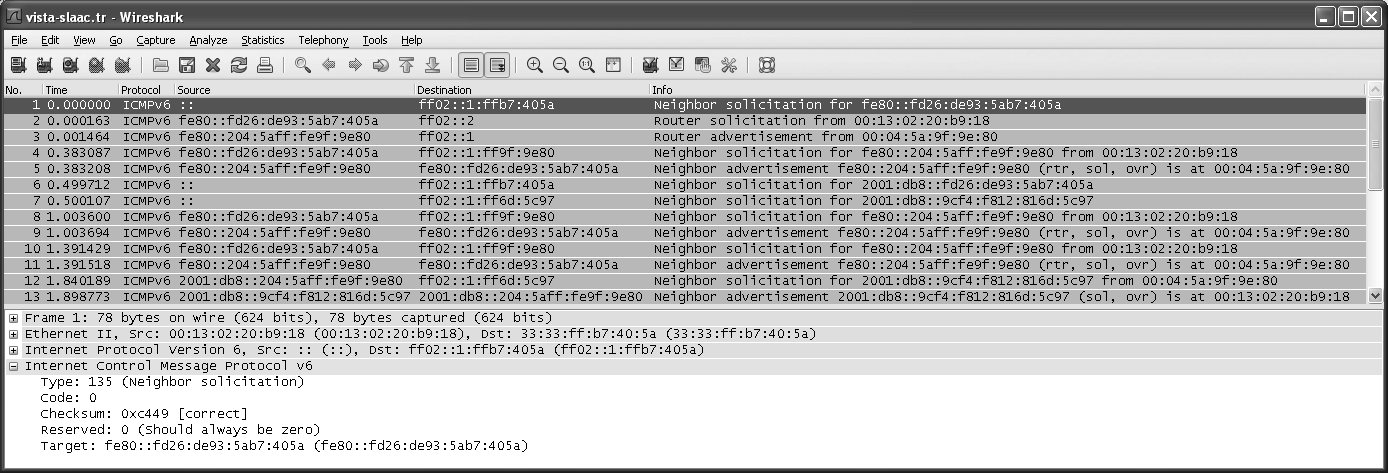
\includegraphics[scale=0.5]{imgs/6/6-23.png}
	\caption{路由器请求导致一台临近的路由器发送了一个路由器通告。请求消息被发送到所有路由器地址(ff02::2)}
\end{figure}

\begin{figure}[H]
    \centering
	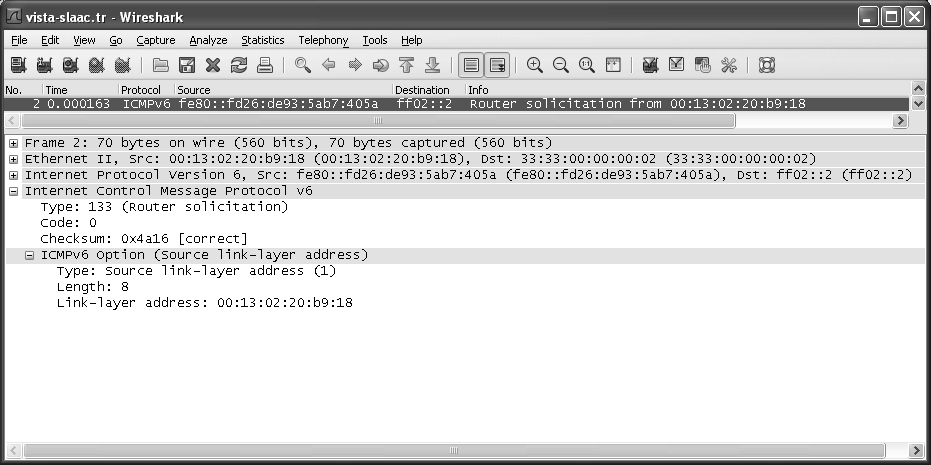
\includegraphics[scale=0.5]{imgs/6/6-24.png}
	\caption{ ICMPv6 RS消息导致一台临近的路由器提供配置信息,例如它所在网络上的全球网络前缀}
\end{figure}

\begin{figure}[H]
    \centering
	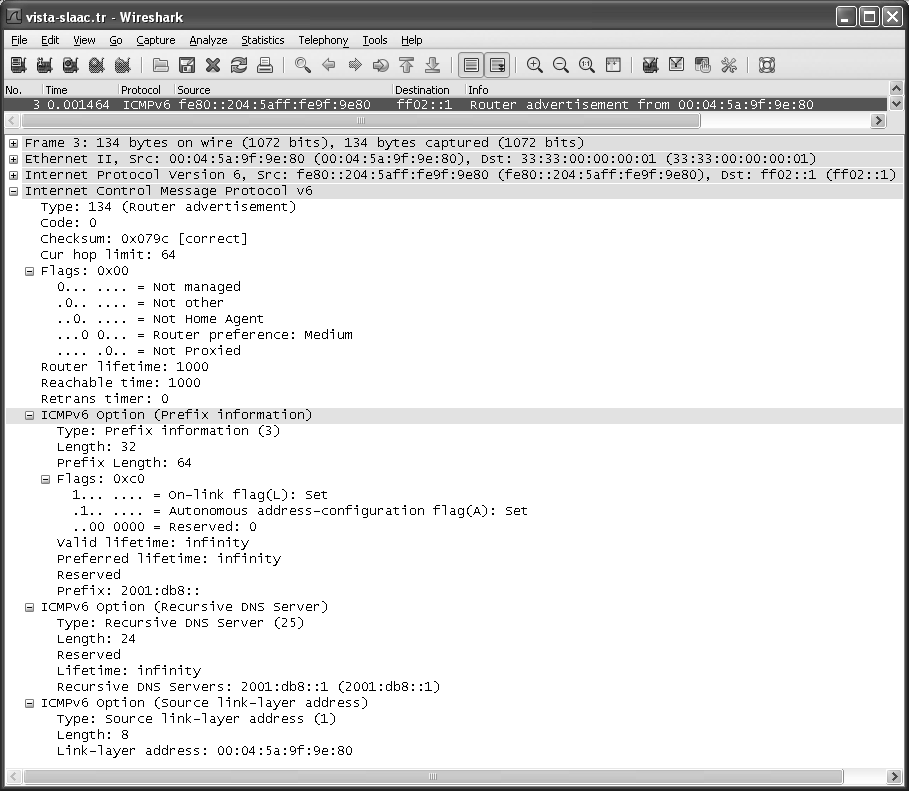
\includegraphics[scale=0.5]{imgs/6/6-25.png}
	\caption{ICMPv6 RA 消息提供了网络中的默认路由器和全局地址前缀的位置以及是否可用的信息。它
    也包括一个 DNS 服务器的位置,并表明该路由器是否可像移动 IPv6 家乡代理(本例中没有)
    那样发送通告。客户机在配置操作中可能使用部分或全部信息}
\end{figure}

\begin{figure}[H]
    \centering
	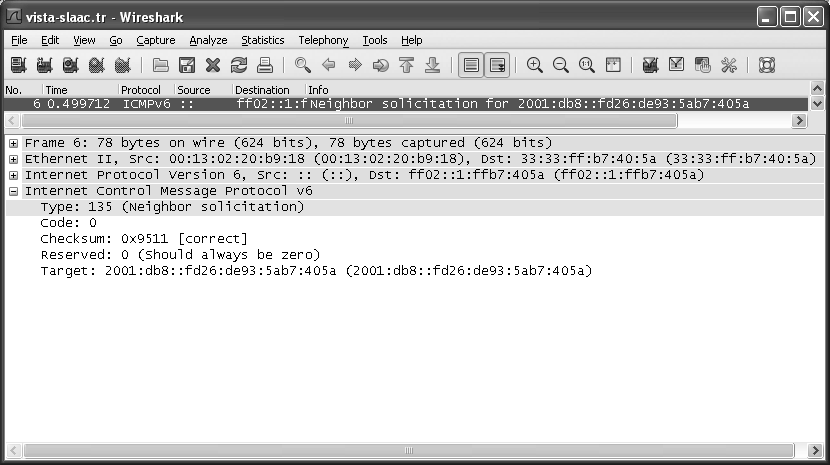
\includegraphics[scale=0.5]{imgs/6/6-26.png}
	\caption{ICMPv6 RA 消息提供了网络中的默认路由器和全局地址前缀的位置以及是否可用的信息。它
    也包括一个 DNS 服务器的位置,并表明该路由器是否可像移动 IPv6 家乡代理(本例中没有)
    那样发送通告。客户机在配置操作中可能使用部分或全部信息}
\end{figure}

\begin{figure}[H]
    \centering
	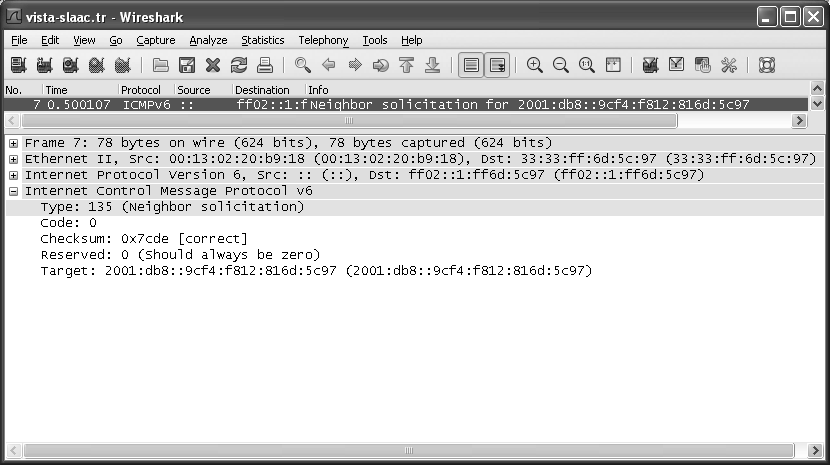
\includegraphics[scale=0.5]{imgs/6/6-27.png}
	\caption{对地址 2001:db8::9cf4:f812:816d:5c97 的 DAD}
\end{figure}

图6-27中的DAD操作针对地址 2001:db8::9cf4:f812:816d:5c97。这个地址是一个临时
IPv6地址,出于隐私保护的原因,它的低序位使用一个不同的随机数来生成。两个全球地址
之间的区别是临时地址的生命周期较短。生命周期是由以下两个值中较小的值计算得到:RA
中接收到的前缀信息选项中包含的生命周期和一对本地默认的生命周期。在 Windows Vista
的例子中,默认的有效生命周期为一星期,而默认的首选生命周期为一天。当这个消息已完
成后,客户机对自己的链路本地地址和两个全球地址执行 SLAAC。通过这些地址信息足以
进行本地或全球通信。临时地址将定期更改,以协助增强隐私保护。在不需要隐私保护的情
况下,可使用以下命令在 Windows 中禁用该功能:


\begin{verbatim}
c:l> netsh interface ipv6 Bet privacy state=disabled
\end{verbatim}

在 Linux 中,使用以下命令启用临时地址:
\begin{verbatim}
Linux# syectl -w net.ipv6.cont.al1.u8e\_tempaddr=2
Linux# sysctl -w net.ipv6.conf.default.use\_tempaddr=2
\end{verbatim}

使用以下命令禁用临时地址:
\begin{verbatim}
Linux# aysct1 -w net.ipv6.conf.a11.use\_tempaddr=0

Linux# sysctl -w net.ipv6.conf.default.use\_tempaddr=0
\end{verbatim}

\subsubsection{无状态 DHCP}
我们已提到 DHCPv6 可用于一种“无状态”模式,在这种模式下,DHCPv6服务器不
指定地址(或保留任何一台客户机的状态),但提供其他配置信息。无状态 DHCPv6定义在
\href{https://www.rfc-editor.org/rfc/rfc3736}{\href{https://www.rfc-editor.org/rfc/rfc3736}{[RFC3736]}} 中,并将SLAAC 和 DHCPv6 相结合。有人认为这种结合是一种有吸引力的部署
方案,网络管理员在部署 DHCPv4 时不必直接关心地址池。

在一个无状态 DHCPv6 部署方案中,假设节点采用DHCPv6之外的方法获得自己的地
址。因此,DHCPv6 服务器不需要处理定义在表6-1中的地址管理消息。另外,它不需要处理
建立IA 绑定所需的选项。这大大简化了服务器软件和配置工作。中继代理的操作没有改变。

无状态 DHCPv6 客户机使用 DHCPv6的 INFORMATION-REQUEST消息请求信息,该
信息由服务器发送的 REPLY 消息提供。INFORMATION-REQUEST 消息包含一个选项请求
选项,给出客户机想了解的更多信息的选项。INFORMATION-REQUEST 可能包含一个客户
机标识符选项,它允许为特定的客户机定制答案。

为了实现标准的无状态DHCPv6服务器,相应系统必须实现以下这些消息:
INFORMATION-REQUEST、REPLY、RELAY-FORW 和 RELAY-REPL。它还必须实现以下
这些选项:选项请求、状态代码、服务器标识符、客户机消息、服务器消息和接口 ID。最后
三个选项在作为中继代理时使用。作为一台可用的无状态 DHCPv6服务器,其他几个选项可
能是必要的:DNS服务器、DNS 搜索列表和可能的SIP服务器。其他可能有用但不是必需
的选项主要包括:优先级、经历的时间、用户类别、供应商类别、供应商特定信息、客户机
标识符和认证。

\subsubsection{地址自动配置的用途}
IP 地址自动配置的用途通常是有限的,这是由于路由器可能需要为同一网络中的客户机
配置特定范围的IP地址,而这台客户机自动配置的地址与该范围不一致。它在IPV4(APIPA)
环境中是好用的,这是因为专用链路本地前缀169.254/16 不能用于路由器中。因此,自己分
配IP 地址的结果是本地子网访问可能正常,但 Internet 路由和名称服务(DNS)很可能不正
常。当DNS 不正常时,大部分常见 Internet“体验”无法实现。因此,一台客户机无法获得一
个IP地址(相对容易检测),相对于获得一个实际不能有效使用的IP 地址,前者通常更有用。

\begin{tcolorbox}
    其他可能用于链路本地编址的名字服务包括Bonjour/ZeroConf (Apple)、
    LLMNR 和 NetBIOS(Microsoft)。随着时间推移,这些来自不同厂商的服务没有成
    为IETF标准,在本地环境中将名称映射到地址时的行为有很大差别。关于DNS本
    地替代者的详细信息见第11章。
\end{tcolorbox}

我们可以禁止使用 APIPA,防止系统自己分配一个 IP地址。在Windows 中,这是通过
创建以下注册表项(注册表项是一行,这里为了说明而换了行)来完成:

\begin{verbatim}
    
HKLM\SYSTEM\CurrentControlSet \Services \Tcpip\Parameters\
IPAutoconfigurationEnabled
\end{verbatim}

REG\_DWORD 值可设置为O,对所有网络接口禁用 APIPA。在Linux 中,文件/etc/
sysconfig/network 可修改为包括以下指令:

NOZEROCONE=YeS

这将禁止所有网络接口使用 APIPA。通过修改每个接口的配置文件(例如,第一个以太
网设备的 /etc/sysconfig/network-scripts/ifcfg-ethO),也可禁止特定接口使用 APIPA。

在 IPv6 SLAAC 的情况下,获得一个全局 IPv6地址相对容易,但一个名称和其地址之
间的关系并不安全,从而导致潜在的安全问题(参见第11章和第18章)。因此,在部署中暂
时仍希望避免使用SLAAC。对IPv6 全局地址禁用SLAAC 有两种方法。首先,在本地路由
器提供的路由器通告消息的前缀选项中关闭“自动”标志(配置不提供前缀选项,如前面
的例子中所示)。另外,可通过本地配置来避免客户机进行全局地址的自动配置。

在一台 Linux 客户机中禁用 SLAAC,可使用以下命令:

\begin{verbatim}    
Linux# sysct1 -w net.ipv6.conf.all.autoconf=0
\end{verbatim}

在 Mac OS或 FreeBSD 系统中禁用SLAAC(至少是针对本地链路地址),可使用以下
命令:

\begin{verbatim}
FreeBSD#

sysctl -w net.inet6.ip6.auto\_1ink1oca1=0
\end{verbatim}
而 Windows 系统中的相应禁用命令为:

\begin{verbatim}
C:\> netsh
netsh> intertace ipv6
netsh interface ipv6> get interface {ifname}managedaddress=disabled
\end{verbatim}

其中,{fname}应替换为相应接口的名称(在这个例子中是“Wireless Network
Connection”)。注意,随着时间推移,这些配置命令的行为有时会发生变化。如果这些变化
没有如预期那样执行,请查看针对当前方法的操作系统文件。

\section{DHCP 和 DNS 交互}
当一台 DHCP 客户机获得一个 IP 地址时,它接收的配置信息的重要部分是一台 DNS
服务器的IP地址。它允许客户机系统将 DNS名称转换IPv4 和/ 或IPv6地址,该地址是
进行传输层连接时协议实现所需要的。如果没有DNS服务器或其他方式将域名映射为IP
地址,大多数用户会发现他们几乎难以访问互联网系统。如果本地 DNS工作正常,它将
Internet 作为一个整体来提供地址映射,但如果配置正确,也可针对本地的专用网络(如前面
提到的.home)。

由于本地专用网络的DNS映射通常采用烦琐的手工管理,因此,将指定 DHCP地址与
相应地址的 DNS映射更新方法结合起来将会带来方便。这可通过组合DHCP/DNS 服务器或
动态 DNS(见第11章)来实现。

组合 DNS/DHCP 服务器(如 Linux dnsmasqg 包)是一个服务器程序,它可配置为提供IP
地址租约以及其他信息,也可读取一个 DHCPREOUEST 中的客户机标识符或域名,并在使
用DHCPACK 进行响应之前,通过“名称到地址”的绑定更新内部DNS 数据库。这样,由
DHCP客户机或与相同 DNS服务器交互的其他系统发起的任何后续 DNS 请求,能够在客户
机名称和新分配的IP 地址之间转换。

\section{以太网上的 PPP}

对于大多数局域网和一些广域网连接,DHCP 提供了最常用的客户机系统配置方法。
对于广域网连接(例如 DSL),常用另一种基于 PPP 的方法代替它。这种方法涉及在以太网
中携带 PPP,因此称为以太网上的 PPP(PPPoE)。PPPoE 用于广域网连接设备(例如 DSL
调制解调器)作为一个交换机或网桥而不是使用路由器的情况下。PPP 作某些ISP 建立连
接的首选,这是因为它可提供比其他配置选项(例如 DHCP)更细致的配置控制和审计日
志。为了提供Internet 连接,有些设备(例如用户PC)必须实现IP路
由和寻址功能。图6-28显示了典型的使用情况。

IsP

该图显示了一个ISP使用 DSL

为很多客户提供服务。DSL 提供一

接入集中器

条点到点的数字链路,它可与一条

点到点

以太网

家用PC

电话网络

传统的模拟电话线(称为普通老式电

话业务或POTS)同时工作。对物理

网桥

电话线的同时使用是通过频分复用

来实现的,DSL信息在比POTS更

来自电话

公司的线路

高的频率上传输。当连接到传统的

終 6-28

为客户提供使用PPPoE 的DSL服务的简化视图。

电话听筒时,需要用一个过滤器来

避免更高的DSL 频率的干扰。DSL

家用PC实现了PPPoE协议,并向ISP进行用户

调制解调器次PPP端口提供桥接服

身份认证。它也可作为家乡局域网中的路由器、

DHCP 服务器、DNS服务器或 NAT 设备

务,该端口位于ISP 的接入集中器

(AC)中,连接客户的调制解调器线和ISP的网络设备。调制解调器和 AC也支持PPPOE 协
议,在这个例子中,该用户选择将一台家用PC连接到DSL 调制解调器,并使用一个点到点
的以太网络(即仅使用一根电缆的以太网)。

在DSL 调制解调器与ISP成功建立一条低层链路后,PC可以开始进行 PPPoE交换,它

被定义在信息文档\href{https://www.rfc-editor.org/rfc/rfc2516}{\href{https://www.rfc-editor.org/rfc/rfc2516}{[RFC2516]}}中,如图6-29所示。

这个协议包括一个发现阶段和一个 PPP会话阶段。发现阶段涉及交换几个 PPPOE主动

发现(PAD)消息:PADI(初始化)、PADO(提供)、PADR(请求)和PADS(会话确认)。
在这个交换完成后,由以太网封装的一次 PPP会话开始,并最终由任何一方发送 PADT(终
止)消息来终止。如果低层连接中断,这个会话也会终止。PPPoB 消息使用图6-30所示的格
式,并封装在以太网的有效载荷区。

在图6-30中,PPPOE版本和类型字段的长度都是4位,并包含当前 PPPoE版本的值

0x1。代码字段中包含 PPPoE消息类型的提示,如图 6-30的右下部分所示。会话ID 字段包
含值0x0000表示 PADI、PADO 和PADR消息,并在后续消息中包含一个唯一的16位数字。
在PPP 会话阶段会保持相同的值。PAD 消息包含一个或多个标签,它们按 TLV 方式排列为
200

第6章

一个16位的TAG\_TYPE字段,随后是一个16位的TAG\_LENGTH 字段和一个数据可变的

标签值。表6-2给出了 TAG\_TYPE 字段的值和含义。

对等方 1

(客户机)

对等方 2

(服务器)

交换的消息

发现

PADI

(广播)

PADO

一(单播)

提供

选择

PADR

(单播)

最新网络工程师资料

www.w.gcs.cn

准备

PADS

(单播)

PPP会话

关闭

PADT

(单播)

关闭

图 6-29
PPPoE 消息交换开始于发现阶段及建立 PPP会话阶段。每个消息是一个 PAD 消息。PADI 请
求来自 PPPoE服务器的响应。PADO 提供连接。PADR 表示客户机可以从多个可能的服务器
中做出选择。PADS从选中的服务器向客户机提供一个确认。经过 PAD交换,一次PPP会话
开始。PPP会话可由任何一方发送 PADT 消息来终止,或在低层链路出现故障时关闭
将 PPPoE 的版本设置力Ox1

0

1516

31

版本

(4位)

会话 ID

(16位,发现阶段的值为0)

类型

(4位)

代码

(8位)

长度

(16位,有效载荷的长度)

图 6-30

287

288

有效载荷(可变)

[PAD 消息在有效载荷区中包含 TLV 标签]

PPPoE 以太网类型

0x8863(发现)

0x8864(PPP 会话)

代码值

0x09 (PADI)

0x07 (PADO)

0x19(PADR)

0x65(PADS)

0xA7 (PADT)

0x00(PPP 会话)

PPPoE 消息携带在以太网帧的有效载荷区。以太网类型字段在发现阶段设置为Ox8863,而设
置为 0x8864 表示携带 PPP 会话数据。对于 PAD 消息,采用TLV 方式携带配置信息,这类似
于 DHCP 选项。服务器选择一个 PPPoE 会话 ID,并在 PADS 消息中传输

表 6-2

值

0x0000

0x0101

0x0102

0x0103

0x0104

0×0105

0x0110

0x0201

0x0202

0x0203

PPPOE 的TAG\_TYPE 字段的值、名称和用途。PAD消息可能包含一个或多个标签

名称

End-of-List

Service-Name

AC-Name

Host-Uniq

AC-Cookie

Vendor-Specific

Relay-Session-ID

Service-Name-Error

AC-System-Error

Generic-Error

用途

表示没有更多标签存在。TAG\_LENGTH必须为0

包含一个UTF-8编码的服务名称(供ISP 使用)

包含一个 UTF-8编码的字符串,用于表示访问集中器

由客户机使用的二进制数据,用于匹配消息;不能被AC解释

由AC使用的二进制数据,用于防止 DoS;由客户机回显

不推荐;更多细节见\href{https://www.rfc-editor.org/rfc/rfc2516}{\href{https://www.rfc-editor.org/rfc/rfc2516}{[RFC2516]}}

中继增加该值以转发 PAD流量

请求的 Service-Name 标签不能被AC认可

AC 在执行请求的操作时出现一个错误

包含一个 UTF-8编码的字符串,用于描述一个不可恢复的错误

为了查看PPPoE的行为,我们可监控图6-28所示的一个家用系统(例如家用 PC)与一
台接人集中器之间的数据交换。图6-31显示了发现阶段和第一次 PPP会话数据包。

图6-31显示了预期的PADI、PADO、PADR 和PADS消息交换。每个消息包含一个
值为9c3a0000的Host-Uniq 标签。来自集中器的消息也包含一个值为90084090400368-
rback37.snfcca 的AC-Name 标签。图6-32显示了PADS消息的详细信息。

在图6-32中,PADS消息表示为客户机建立一次PPP会话,并使用 Oxecbd 作为会话
ID。AC-Name 标签仍然保持,表示使用原来的AC。至此,发现阶段已完成,可开始一次普
通的PPP会话(见第3章)。图6-33显示了第一次 PPP会话的数据包。

该图说明 PPPoE交换中的PPP会话阶段开始。PPP 会话开始于链路配置(PPP LCP),
这里由客户机发送一个配置请求(见第3章)。它表明客户机想使用密码认证协议(一种相对
不安全的方法)向AC认证自己。当认证交换已完成,并交换了各种链路参数(例如 MRU),
IPCP 用于获取和配置 IP 地址。注意,这时可能需要额外的配置信息(例如,ISP的 DNS服
务器的IP 地址),它取决于ISP的配置(即手工配置)。

\section{与系统配置相关的攻击}

针对系统和网络配置的攻击多种多样。从未授权客户机或未授权服务器对 DHCP 的干
扰,到耗尽资源的各种形式的DoS攻击,例如申请一台服务器可能提供的所有可能的IP地
址。这些问题很常见,这是由于地址配置基于旧的IPv4 协议,其设计出发点是假设网络可
信,而到目前为止新的协议还很少部署(安全部署就更少见)。因此,无法通过典型DHCP
部署来防御这些攻击,虽然链路层认证(例如,Wi-Fi 网络使用的WPA2)有助于限制连接
到一个特定网络的未授权客户机数量。

IETF 致力于IPv6邻居发现提供安全性,哪个邻居、什么时间或是否已部署SLAAC,
这些因素将直接影响网络运行的安全性。\href{https://www.rfc-editor.org/rfc/rfc3756}{\href{https://www.rfc-editor.org/rfc/rfc3756}{[RFC3756]}} 概括了2004年以米的信任及威胁假设,
\href{https://www.rfc-editor.org/rfc/rfc3971}{\href{https://www.rfc-editor.org/rfc/rfc3971}{[RFC3971]}}定义了安全邻居发现(SEND)协议。SEND 将 IPsec(见第18章)用于邻居发现
数据包,并结合使用加密生成的地址(CGA)\href{https://www.rfc-editor.org/rfc/rfc3972}{\href{https://www.rfc-editor.org/rfc/rfc3972}{[RFC3972]}}。这种地址由密钥散列函数而获得
所以它们只能由系统保存的适当关键信息生成。

\begin{figure}[H]
    \centering
	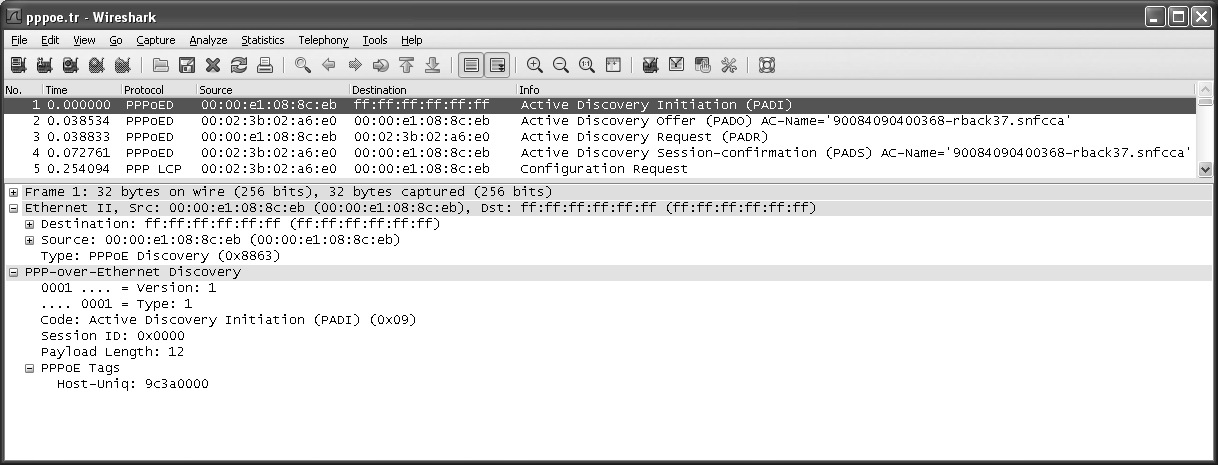
\includegraphics[scale=0.5]{imgs/6/6-31.png}
	\caption{对地址 2001:db8::9cf4:f812:816d:5c97 的 DAD}
\end{figure}

\begin{figure}[H]
    \centering
	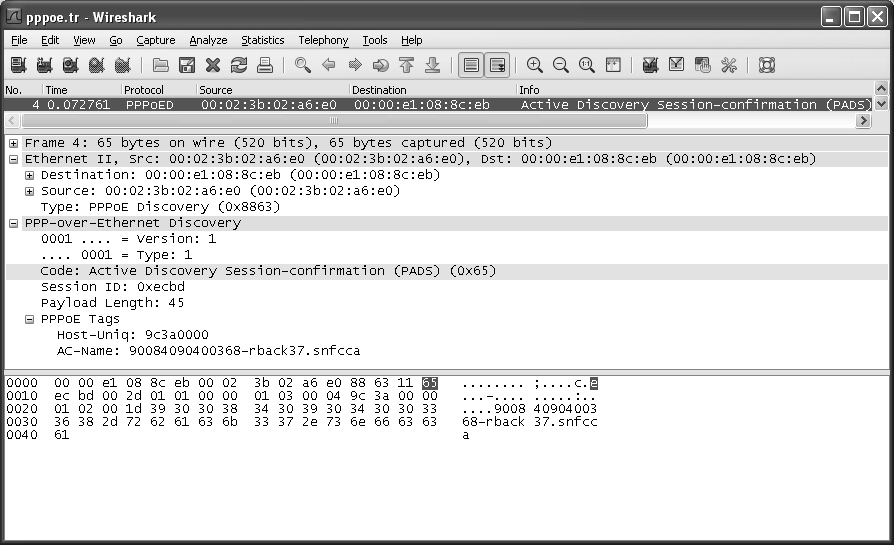
\includegraphics[scale=0.5]{imgs/6/6-32.png}
	\caption{PPPoE的PADS消息用于确认客户机和接人集中器之间的关联。这个消息
    还将会话ID设置为Oxecbd,它用于后续PPP会话数据包中}
\end{figure}

\begin{figure}[H]
    \centering
	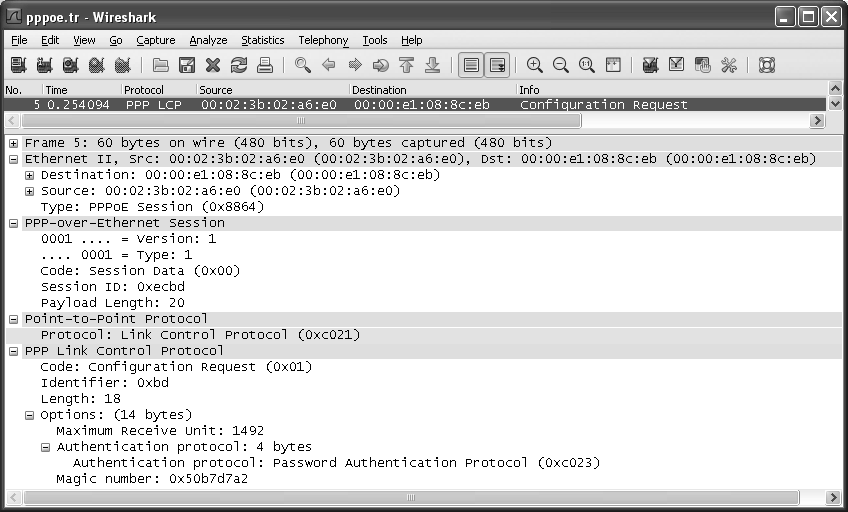
\includegraphics[scale=0.5]{imgs/6/6-33.png}
	\caption{PPPOE 会话的第一个 PPP消息是一个配置请求。以太网类型更改为Ox8864,表示这是一?
    动的PPP会话,并且会话ID 设置为Oxecbd。在这个例子中,PPP客户机使用相对不安
    密码认证协议进行身份认证}
\end{figure}

\section{总结}

主机或路由器使用 Internet 协议在 Internet 或专用网络中运行时需要一组基本的配号
路由器通常至少需要分配寻址信息,而主机需要地址、下一跳路由器和DNS服务名
位置。DHCP 可同时用于IPv4 和 IPv6,但两者之间不能直接互操作。通过DHCP,适当配
置的服务器可向请求的客户机分配一个或多个地址,并让它们租用一段时间。如果客户机想
继续使用该地址,它可更新自己的租约。客户机也可通过 DHCP 获得更多信息,例如子网掩
码、默认路由器、供应商的特定配置信息、DNS服务器、家乡代理和默认域名。当客户机和
服务器位于不同网络中,可通过中继代理使用DHCP。当使用中继代理时,一些 DHCP扩展
允许在中继代理和服务器之间携带额外信息。DHCPv6也可用于为一台路由器委托一个 IPv6
地址空间范围。

一台IPv6主机通常使用多个地址。IPv6客户机能自主生成自己的链路本地地址,这是
通过将一个特定的链路本地IPv6前缀与其他本地信息(例如从自己的MAC地址中获得的
特殊位或有助于保护隐私的随机数)相结合来实现的。要获得一个全局地址,客户机可从
ICMP 路由器通告消息或 DHCPv6服务器获得一个全球地址前缀。DHCPv6 服务器可工作在
“有状态”模式,为请求的客户机提供 IPv6地址租用;它也可工作在“无状态”模式,提供
地址之外的其他配置信息。

PPPoE 协议通过以太网携带 PPP 消息以与ISP 建立 Internet 连接,特别是那些使用DSL
提供服务的ISP。当使用PPPoE 时,用户通常有一台带以太网端口的DSL 调制解调器,该
端口就像一个网桥或交换机。PPPoE首先交换一组发现消息,以确定一个访问控制器的身份,
并建立一次 PPP会话。在发现阶段完成后,PPP流量可封装在以太网帧中,并携带不同协议
(例如IP),这可能持续到 PPPoE会话终止(不管是有意为之还是因为低层链路断开)。当使
用 PPPoE时,PPP协议配置功能,例如IPCP(在第3章中讨论),最终负责为客户机分配IP
地址。

用于IPv6无状态自动配置的DHCP 和ICMPv6 路由器通告,部署时通常没有使用安全
机制。由于这个原因,它们很容易受到一些攻击,包括未授权客户机的网络访问、生成伪造
地址的欺骗性DHCP服务器和各种形式的拒绝服务,以及客户机请求的地址超过可用地址的
资源耗尽攻击等。大多数攻击可通过为DHCP 增加安全机制来缓解,例如 DHCP 认证和最
近出现的SEND协议。但是,它们目前仍很少使用。

\section{参考文献}

[802.21-2008] 'IEEE Standard for Local and Metropolitan Area Networks—Part

21: Media Independent Handover Services,” Nov.2008.

[F07] R. Faas, "Hands On: Configuring Apple's NetBoot Service, Part 1./ Comput-

erworld, Sept. 2007.

[GC89] C. Gray and D. Cheriton, "Leases: An Efficient Fault-Tolerant Mechanism

for Distributed File Cache Consistency." Proc. ACM Symposium on Operating Sys-

tem Principles(SOSP),1989.

IARP http://www.iana.org/assignments/arp-parameters

[IBDP] http://www.iana.org/assignments/bootp-dhcp-parameters

[ID4LQ] K. Kinnear, B. Volz, M. Stapp, D. Rao, B. Joshi, N. Russell, and P. Kurapati,

“Bulk DHCPV Lease Query" Internet draft-ietf-dhc-dhcpv4-bulk-leasequery,

work in progress, Apr. 2011.

[ID4RI] B.Joshi, R. Rao, and M. Stapp, "The DHCPv4 Relay Agent Identifier Sub-

Option" Internet draft-ietf-dhc-relav-id-suboption, work in progress, June 2011.

统配置:DHCP 和自动配置

[ID6PARAM] http://www.iana.org/assignments/dhcpv6-parameters

[IDDN]G. Daley, E. Nord mark, and N. Moore, "Tentative Options for Link-

Layer Addresses in IPv6 Neighbor Discovery," Internet draft-ietf-dna-tentative

(expired), work in progress, Oct. 2009.

[IDL.2RA] B. Joshi and P. Kurapati, "Layer 2 Relay Agent Information," Internet
draft-ietf-dhc-I2ra, work in progress, Apr. 2011.

[IEPARAM] http://www.iana.org/assignments/enterprise-numbers

[MKB928233] Microsoft Knowledge Base Article 928233 at http://support

.microsoft.com

[MS-DHCPN] Microsoft Corporation, "[MS-DHCPN]: Dynamic Host Configura
tion Protocol (DHCP) Extensions for Network Access Protection (NAP)." http://
msdn.microsoft.com/en-us/library/cc227316.aspx, Oct. 2008.